\documentclass[11pt]{article}

% Change "review" to "final" to generate the final (sometimes called camera-ready) version.
% Change to "preprint" to generate a non-anonymous version with page numbers.
\usepackage[review]{acl}

% Standard package includes
\usepackage{times}
\usepackage{latexsym}

% For proper rendering and hyphenation of words containing Latin characters (including in bib files)
\usepackage[T1]{fontenc}
% For Vietnamese characters
% \usepackage[T5]{fontenc}
% See https://www.latex-project.org/help/documentation/encguide.pdf for other character sets

% This assumes your files are encoded as UTF8
\usepackage[utf8]{inputenc}

% This is not strictly necessary, and may be commented out,
% but it will improve the layout of the manuscript,
% and will typically save some space.
\usepackage{microtype}

% This is also not strictly necessary, and may be commented out.
% However, it will improve the aesthetics of text in
% the typewriter font.
\usepackage{inconsolata}

%Including images in your LaTeX document requires adding
%additional package(s)
\usepackage{graphicx}
\usepackage{multirow}
\usepackage{xcolor}
\usepackage{amssymb}
\usepackage{booktabs}
\usepackage{natbib}
% If the title and author information does not fit in the area allocated, uncomment the following
%
%\setlength\titlebox{<dim>}
%
% and set <dim> to something 5cm or larger.

\title{EduIllustrate: An Agentic Pipeline for Generating Diagram-Rich Explanations of K-12 STEM Problems}

% Author information can be set in various styles:
% For several authors from the same institution:
% \author{Author 1 \and ... \and Author n \\
%         Address line \\ ... \\ Address line}
% if the names do not fit well on one line use
%         Author 1 \\ {\bf Author 2} \\ ... \\ {\bf Author n} \\
% For authors from different institutions:
% \author{Author 1 \\ Address line \\  ... \\ Address line
%         \And  ... \And
%         Author n \\ Address line \\ ... \\ Address line}
% To start a separate ``row'' of authors use \AND, as in
% \author{Author 1 \\ Address line \\  ... \\ Address line
%         \AND
%         Author 2 \\ Address line \\ ... \\ Address line \And
%         Author 3 \\ Address line \\ ... \\ Address line}

\author{First Author \\
  Affiliation / Address line 1 \\
  Affiliation / Address line 2 \\
  Affiliation / Address line 3 \\
  \texttt{email@domain} \\\And
  Second Author \\
  Affiliation / Address line 1 \\
  Affiliation / Address line 2 \\
  Affiliation / Address line 3 \\
  \texttt{email@domain} \\}

%\author{
%  \textbf{First Author\textsuperscript{1}},
%  \textbf{Second Author\textsuperscript{1,2}},
%  \textbf{Third T. Author\textsuperscript{1}},
%  \textbf{Fourth Author\textsuperscript{1}},
%\\
%  \textbf{Fifth Author\textsuperscript{1,2}},
%  \textbf{Sixth Author\textsuperscript{1}},
%  \textbf{Seventh Author\textsuperscript{1}},
%  \textbf{Eighth Author \textsuperscript{1,2,3,4}},
%\\
%  \textbf{Ninth Author\textsuperscript{1}},
%  \textbf{Tenth Author\textsuperscript{1}},
%  \textbf{Eleventh E. Author\textsuperscript{1,2,3,4,5}},
%  \textbf{Twelfth Author\textsuperscript{1}},
%\\
%  \textbf{Thirteenth Author\textsuperscript{3}},
%  \textbf{Fourteenth F. Author\textsuperscript{2,4}},
%  \textbf{Fifteenth Author\textsuperscript{1}},
%  \textbf{Sixteenth Author\textsuperscript{1}},
%\\
%  \textbf{Seventeenth S. Author\textsuperscript{4,5}},
%  \textbf{Eighteenth Author\textsuperscript{3,4}},
%  \textbf{Nineteenth N. Author\textsuperscript{2,5}},
%  \textbf{Twentieth Author\textsuperscript{1}}
%\\
%\\
%  \textsuperscript{1}Affiliation 1,
%  \textsuperscript{2}Affiliation 2,
%  \textsuperscript{3}Affiliation 3,
%  \textsuperscript{4}Affiliation 4,
%  \textsuperscript{5}Affiliation 5
%\\
%  \small{
%    \textbf{Correspondence:} \href{mailto:email@domain}{email@domain}
%  }
%}

\begin{document}
\maketitle
\begin{abstract}
Generating high-quality illustrated explanations for K-12 STEM problems requires both geometrically accurate diagrams and coherent step-by-step reasoning---a combination that existing LLM-based educational content systems have not addressed. We present \textbf{EduIllustrate}, an automated four-stage agentic pipeline that takes a K-12 STEM problem as input and produces a structured, diagram-rich explanation with programmatically rendered static diagrams via Manim. Our pipeline introduces a sequential anchoring strategy: Scene 1 undergoes full implementation planning to establish visual conventions (color scheme, label formatting, spatial layout), while subsequent scenes generate in parallel conditioned on Scene 1's code, enforcing cross-diagram consistency without global optimization. To enable systematic evaluation, we construct a benchmark of \textbf{118 problems} spanning three grade levels (elementary, middle, high school) and five subjects (mathematics, physics, chemistry, biology, geography), and propose an \textbf{8-dimension evaluation rubric} grounded in multimedia learning theory covering both text quality and visual quality. Evaluation of five frontier LLMs shows Gemini 3.0 Pro Preview achieves the highest overall score (4.40/5.0), while Kimi-K2.5 offers the best cost-efficiency (4.07 at \$0.15/problem). Workflow ablation confirms our sequential anchoring improves visual consistency (D6) by 12\% over a fully parallel baseline at 17.5\% lower cost. Human evaluation with 20 expert raters validates LLM-as-judge reliability for objective dimensions ($\rho=0.89$ for logical coherence, $\rho=0.83$ for diagram-problem alignment), while revealing limitations on subjective visual assessment.
\end{abstract}


\section{Introduction}

High-quality illustrated explanations are fundamental to K-12 STEM pedagogy. Research in educational psychology demonstrates that combining textual reasoning with visual diagrams significantly enhances conceptual understanding, particularly for abstract scientific concepts and mathematical problem-solving~\citep{mayer2001multimedia}. However, producing such multimodal educational content at scale remains labor-intensive, requiring both deep domain expertise and technical proficiency in diagram creation tools.

Recent advances in large language models (LLMs) have enabled remarkable progress in generating educational content. \citet{liu2025cogent} demonstrated curriculum-aligned content generation for grade-appropriate science passages, while \citet{wang2025genmentor} introduced goal-oriented personalized learning frameworks powered by multi-agent LLM systems. Programmatic content generation has also advanced: \citet{ku2025theoremexplain} generate long-form theorem explanation videos (over 5 minutes) using Manim animations for university-level mathematics, achieving 93.8\% success rates with videos up to 10 minutes long, while \citet{chen2025code2video} create educational videos via executable Python code for programming tutorials, introducing the TeachQuiz metric for knowledge recovery assessment.

Yet a critical gap remains for \textbf{K-12 STEM education}: existing video generation approaches target university-level theorems or programming content with long-form animated explanations, while K-12 problem explanations require \textbf{static, geometrically accurate diagrams} seamlessly integrated with step-by-step reasoning across diverse subjects (mathematics, physics, chemistry, biology, geography). Unlike long-form videos designed for theorem proofs, K-12 pedagogy emphasizes textbook-style static illustrations that learners can process at their own pace, aligned with grade-appropriate curriculum standards. Moreover, no unified benchmark exists to jointly evaluate textual reasoning quality and visual diagram quality across K-12 STEM disciplines with their subject-specific conventions.

This gap is particularly pronounced because K-12 STEM diagrams carry precise semantic meaning: geometry proofs require exact angle measurements and spatial relationships; physics problems demand force vectors with correct directions and magnitudes; chemistry explanations need molecular structures following discipline-specific conventions. Generating such diagrams programmatically introduces challenges in geometric accuracy, visual consistency across multiple diagrams, semantic alignment between text and visuals, and developing evaluation frameworks capturing both perceptual quality and pedagogical effectiveness.

We address these challenges with \textbf{EduIllustrate}, an automated four-stage pipeline generating illustrated K-12 STEM explanations with programmatically rendered diagrams via Manim. Our system decomposes generation into: (1) structured outline with interleaved text and scene specifications, (2) per-scene implementation planning with explicit spatial constraints, (3) parallel Manim code generation and rendering, and (4) final Markdown assembly. To systematically evaluate multimodal educational content, we construct a benchmark of \textbf{118 K-12 STEM problems} spanning three grade levels and five subjects, proposing an \textbf{8-dimension evaluation rubric} grounded in multimedia learning theory.

\textbf{Our contributions are:}

\begin{enumerate}
\item An automated four-stage pipeline for generating diagram-rich K-12 STEM explanations with explicit geometric accuracy and visual consistency constraints
\item A curated benchmark of 118 problems across 3 grade levels and 5 subjects for standardized multimodal evaluation
\item An 8-dimension evaluation rubric with automated and human protocols grounded in educational psychology
\item Comparative study of four frontier LLMs identifying model-specific strengths and failure modes
\item Validation of LLM-as-judge reliability for multimodal content through correlation analysis with human expert ratings
\end{enumerate}

\section{Related Work}

\subsection{LLMs in Education}

LLM applications in education span intelligent tutoring, automated assessment, and adaptive content generation. \citet{kamalov2025agentic} reviewed agentic workflows in education, highlighting advancements in automated tutoring while noting constraints in adaptability that multi-agent frameworks address. \citet{wang2025genmentor} introduced GenMentor, an LLM-powered multi-agent framework for goal-oriented learning, demonstrating effective skill gap identification and personalized learning path scheduling.

For K-12-specific applications, \citet{liu2025cogent} proposed COGENT, a curriculum-oriented framework generating grade-appropriate content aligned with curriculum standards, controlling reading levels through vocabulary and sentence complexity. \citet{memari2025elementary} synthesized 258 studies in elementary STEM education, finding 45\% focused on intelligent tutoring systems but revealing limited cross-disciplinary integration. Despite these advances, existing work predominantly focuses on text-only explanations or assessment, leaving multimodal content generation for K-12 STEM underexplored.

\subsection{Programmatic Educational Content Generation}

Recent work has explored generating educational content through executable code. \citet{ku2025theoremexplain} introduce an agentic approach for generating long-form theorem explanation videos (over 5 minutes) using Manim animations. The system employs a planner agent for video structuring and a coding agent for Python script generation, targeting university-level mathematics and physics theorems. TheoremExplainBench provides 240 theorems across four STEM disciplines with five automated evaluation metrics assessing factual correctness (accuracy and depth, visual relevance, logical flow) and perceptual quality (element layout, visual consistency). The o3-mini model achieved 93.8\% success rate with overall score of 0.77, though human studies revealed visual layout issues remained the primary challenge.

\citet{chen2025code2video} propose a code-centric agent framework for generating professional educational videos via executable Python code, introducing three collaborative agents (Planner, Coder, Critic) and the TeachQuiz metric that quantifies knowledge recovery by unlearned Vision-Language Models after watching generated videos. The framework achieved 40\% improvement over direct code generation, demonstrating scalability and controllability through programmatic manipulation of renderable environments.

Both systems demonstrate LLMs' capability for programmatic educational content generation but target \textbf{video-based explanations} for advanced topics. Our work differs by focusing on \textbf{static diagram generation} for K-12 problem-solving explanations, where textbook-style illustrations enable self-paced learning. We address grade-appropriate pedagogy across five subjects with subject-specific diagram conventions (right-angle markers in geometry, vector arrows in physics, VSEPR molecular geometry in chemistry).

\subsection{Programmatic Diagram Generation}

Programmatic diagram generation leverages tools like TikZ, Manim, and Matplotlib. \citet{kumar2025diagramir} introduced DiagramIR, an automatic evaluation pipeline for educational math diagrams using intermediate representations of LaTeX TikZ code, demonstrating higher agreement with human raters than LLM-as-judge baselines. \citet{cui2025draw} proposed Draw with Thought, a training-free framework guiding multimodal LLMs to reconstruct scientific diagrams into editable mxGraph XML code through Chain-of-Thought reasoning.

\citet{ni2025viscoder} introduced VisCoder, a fine-tuning approach using the VisCode-200K dataset containing validated plotting code paired with natural language instructions. \citet{reux2025vtikz} evaluate LLMs' ability to customize code while preserving visual coherence, revealing state-of-the-art models struggle to modify code aligned with visual intent.

Our work builds on these foundations by introducing \textbf{domain-specific constraints for educational diagrams}: safe margins, minimum element spacing, white backgrounds, relative positioning, and discipline-specific conventions. We address \textbf{visual consistency across multiple diagrams} through conditional generation where subsequent scenes reference Scene 1's code as a visual anchor, enforcing cross-diagram coherence without requiring global multi-scene optimization.

\subsection{LLM-as-Judge Evaluation}

LLMs as evaluators provide practical alternatives to costly human evaluation. Recent analyses show LLM-as-judge achieves 80\% human agreement at 500$\times$ lower cost~\citep{evidentlyai2025judge}, though systematic biases including position bias and self-preference remain. \citet{lee2025lemaj} revealed in the legal domain that reference-free evaluation protocols correlate better with human expert judgments. \citet{park2025agacci} demonstrated AGACCI framework improves accuracy through distributing specialized evaluation roles across collaborative agents.

Existing LLM-as-judge frameworks focus primarily on text quality evaluation with limited visual quality assessment. Our work extends methodology to multimodal educational content by: (1) decomposing evaluation into text-only and vision-enabled dimensions, (2) implementing geometric mean aggregation across multiple diagrams, and (3) validating automated metrics against 20 human expert raters through Spearman correlation and Krippendorff's alpha.

\subsection{Multi-Modal Learning Theory}

Our evaluation framework is grounded in multimedia learning theories. \textbf{Cognitive Load Theory}~\citep{sweller1988cognitive} posits working memory has limited capacity---effective diagrams reduce intrinsic load by externalizing spatial relationships. \textbf{Dual Coding Theory}~\citep{paivio1971imagery} proposes information is processed through separate verbal and visual channels, with learning enhanced when both engage. \textbf{Multimedia Learning Principles}~\citep{mayer2001multimedia} provide design guidelines including spatial contiguity, temporal contiguity, and coherence.

\citet{ji2025eduvis} demonstrated that coordinating specialized agents for instructional planning, reasoning decomposition, and visualization design substantially improves educational alignment in pedagogical visualization tasks. These frameworks inform our 8-dimension rubric: D1-D2 ensure cognitive accuracy; D4 and D8 align with coherence principles; D3 and D7 operationalize dual coding and spatial contiguity; D5-D6 reduce extraneous load through predictable visual patterns.

\section{Method}

\subsection{Task Definition}

\textbf{Agent Input.} The agent receives a K-12 STEM problem statement in plain text, accompanied by a problem diagram image when the original problem includes visual information (e.g., a geometry figure to analyze, a physics setup to reason about).

\textbf{Agent Output.} The agent outputs a structured Markdown document containing: (1) step-by-step textual explanations with pedagogical scaffolding, and (2) programmatically rendered static PNG diagrams via Manim that are geometrically accurate, visually consistent, and semantically aligned with the textual reasoning.

\subsection{EduIllustrate Agent}

We develop \textbf{EduIllustrate Agent}, a four-stage pipeline that decomposes illustrated explanation generation into sequential stages addressing specific multimodal content creation challenges. Figure~\ref{fig:pipeline} illustrates the complete pipeline.

\begin{figure*}[t]
  \centering
  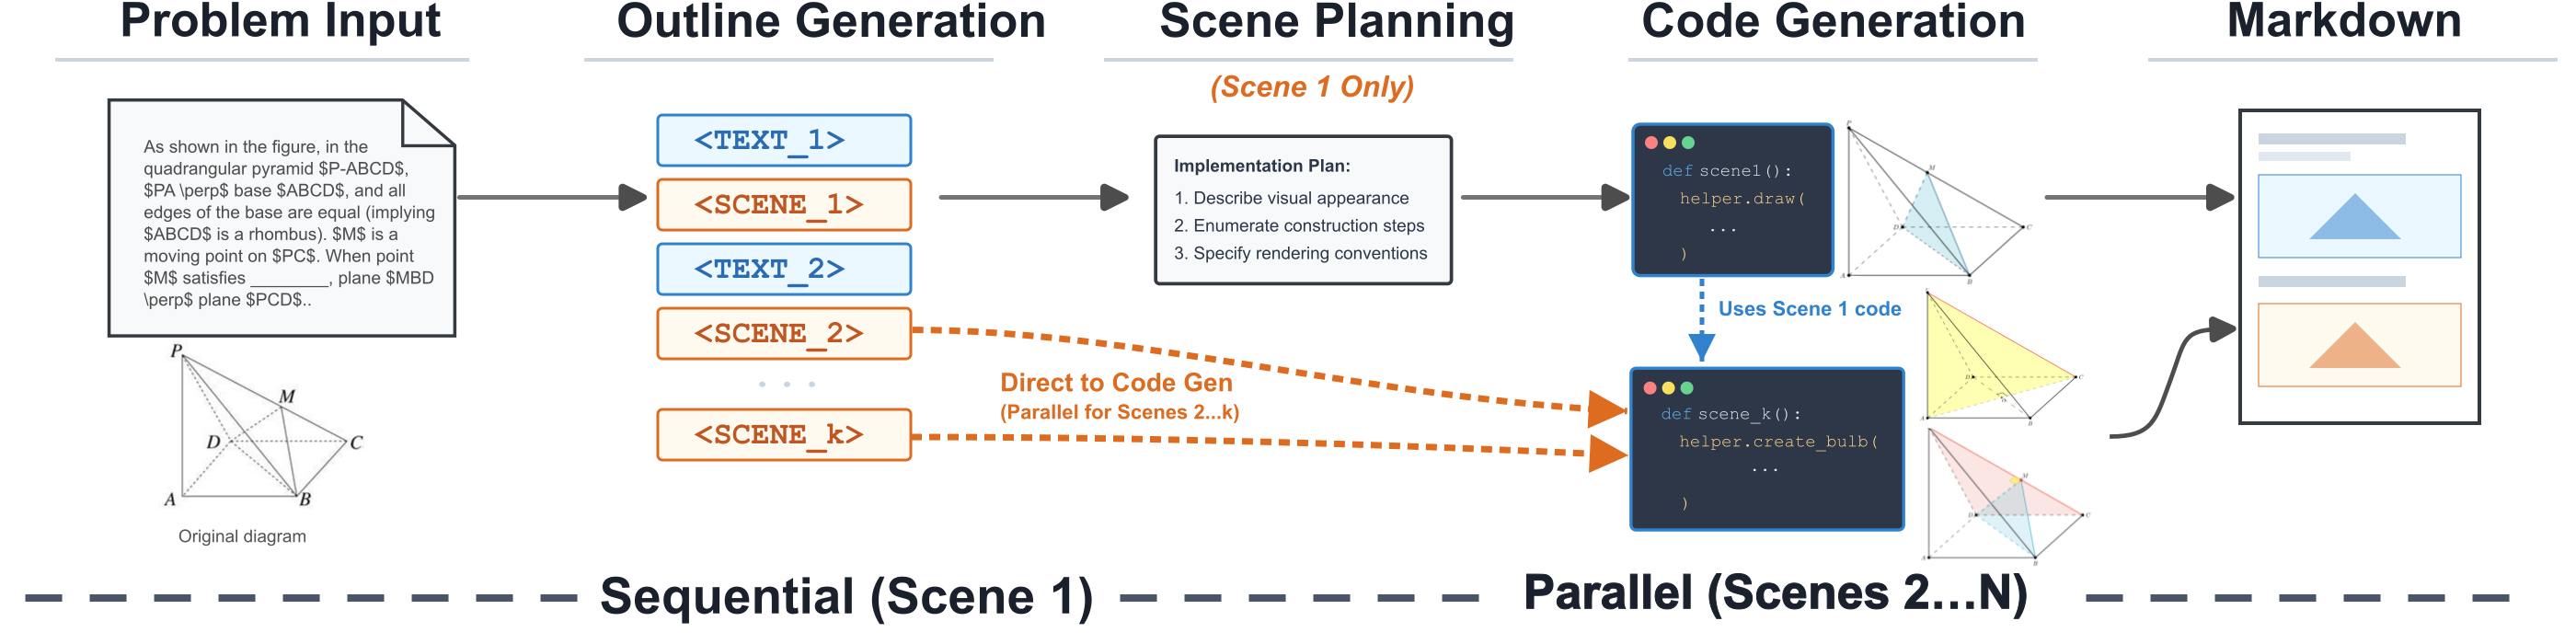
\includegraphics[width=\textwidth]{fig/fig1.png}
  \caption{EduIllustrate pipeline overview. Scene 1 undergoes full sequential processing (outline $\to$ implementation planning $\to$ code generation); Scenes 2--$N$ skip implementation planning and generate in parallel, each conditioned on Scene 1's code as a visual anchor.}
  \label{fig:pipeline}
\end{figure*}

\textbf{Stage 1: Structured Outline Generation.} The first stage transforms raw K-12 STEM problems into structured outlines interleaving textual explanation blocks with visual scene specifications. The model receives the problem statement and optional problem diagram, then outputs an XML-based format with \texttt{<SCENE\_OUTLINE>} tags containing alternating \texttt{<TEXT\_k>} and \texttt{<SCENE\_k>} blocks. Each \texttt{<TEXT\_k>} block contains pedagogical explanation---the first states the problem and solution approach, subsequent blocks provide step-by-step reasoning referencing preceding diagrams, and the final block presents the answer with verification. Each \texttt{<SCENE\_k>} block specifies the scene's learning objective, geometric/domain-specific visual elements, text annotations, color coding, and spatial layout strategy. The model first determines \textbf{diagram necessity}: not all STEM problems benefit from visualization (e.g., purely algebraic manipulations), so \texttt{<SCENE\_k>} blocks are generated only when visual representations genuinely aid conceptual understanding. This structured format enforces pedagogical planning by requiring explicit specification of learning goals and visual strategies before code generation, while enabling modular processing for parallel scene generation and error recovery.

\textbf{Stage 2: Scene Implementation Planning.} The second stage applies exclusively to Scene 1, converting high-level \texttt{<SCENE\_1>} specifications into detailed implementation plans before code generation. This stage addresses translating abstract visual intentions into precise geometric constraints, establishing visual conventions (color scheme, label formatting, line weights, spatial layout) that all subsequent scenes inherit. The implementation plan describes intended visual appearance in natural language, enumerates construction steps with explicit spatial constraints (safe area bounds, minimum element spacing, relative positioning), and specifies discipline-specific rendering conventions (right-angle markers in geometry, vector arrows in physics, VSEPR molecular geometry in chemistry). Making these constraints explicit for Scene 1 reduces ambiguity in the critical anchor scene and provides concrete style reference for parallel generation of remaining scenes.

\textbf{Stage 3: Code Generation and Rendering.} The third stage translates implementation plans into executable Manim code and renders static PNG images, employing a hybrid sequential-parallel strategy balancing visual consistency with computational efficiency. Scene 1 undergoes fully sequential generation---implementation plan followed by code generation---establishing the visual ``anchor'' defining color scheme, labeling conventions, line weights, and font sizes that subsequent scenes maintain. After Scene 1 completes successfully, remaining scenes generate in parallel to reduce latency. Each scene's code generation prompt receives: (1) the scene outline from Stage 1, and (2) Scene 1's complete Manim code as reference for visual style, with explicit instructions to maintain visual consistency by reusing color assignments, label formatting, and layout principles. This conditional generation strategy addresses key limitations of prior single-diagram generation work: while individual diagrams may be geometrically correct, inconsistent visual conventions across multiple diagrams create extraneous cognitive load. By conditioning subsequent scenes on Scene 1's code, we enforce cross-diagram coherence without requiring global multi-scene optimization. Each generated code snippet represents a Manim \texttt{Scene} subclass with a \texttt{construct()} method defining visual elements. We invoke Manim Community Edition with \texttt{-s} flag for static rendering and \texttt{-qh} for high-quality 1080p output. Error handling includes: (1) syntax error detection via Python's \texttt{ast} module before rendering, (2) timeout termination for infinite loops (5-second limit), and (3) rendering failure detection by checking output file existence. Failed scenes trigger single retry with error-augmented prompt; persistent failures result in scene omission with placeholder notice. Static PNG output rather than animations aligns with traditional textbook pedagogy, allowing learners to process visual information at their own pace, as Cognitive Load Theory research suggests animated visualizations can increase extraneous load when learners must simultaneously process temporal changes and spatial relationships~\citep{ji2025eduvis}.

\textbf{Stage 4: Document Assembly.} The final stage assembles complete illustrated explanations into structured Markdown documents interleaving text and diagrams in presentation order. This assembly is deterministic, requiring no LLM involvement. The process extracts \texttt{<TEXT\_k>} blocks from Stage 1 outline in sequential order and interleaves them with rendered scene images using Markdown image syntax, following strict alternating pattern where each text block is followed by its corresponding diagram (when applicable). Each scene image includes alt-text describing visual elements for accessibility. The document includes metadata headers specifying problem source, grade level, subject, and knowledge points. This modular architecture provides: (1) debugging transparency---each stage's output can be inspected independently to diagnose failures, (2) selective regeneration---individual scenes can be regenerated without reprocessing the entire explanation, and (3) format flexibility---the same Stage 1-3 outputs can be assembled into alternative formats (LaTeX, HTML, EPUB) by modifying only Stage 4.

\subsection{EduIllustrate Benchmark}

\textbf{Dataset Construction.} We construct a curated benchmark derived from the K12-Vista dataset~\citep{zhang2025k12vista}, a large-scale repository of Chinese K-12 STEM problems with gold-standard solutions and fine-grained knowledge point annotations. We extract 118 problems following three curation criteria: \textbf{(1) Diagram-Appropriate Problems}---problems where visual representations convey spatial, topological, or relational information essential to problem-solving, rather than merely restating text~\citep{ji2025eduvis}; \textbf{(2) Clear Gold Solutions}---verified step-by-step solutions with intermediate reasoning steps, enabling objective correctness evaluation; \textbf{(3) Diverse Knowledge Points}---sampling to maximize diversity at the 3rd level of K12-Vista's 4-level knowledge point taxonomy, ensuring varied conceptual coverage. The full knowledge point breakdown is provided in Appendix~\ref{sec:benchmark-details}.

The benchmark comprises 118 problems across three grade levels (elementary, middle, high school) and five STEM subjects, as shown in Table~\ref{tab:dataset}. All 118 problems include original diagrams in the problem statement, requiring models to interpret visual input and generate explanatory diagrams that reference or extend the given figure. Problems require 2--6 solution steps (mean = 3.8, SD = 1.2), and collectively span 102 distinct knowledge points at the 3rd taxonomy level.

\begin{table}[t]
\centering
\small
\begin{tabular}{lcccccc}
\hline
\textbf{Grade} & \textbf{Math} & \textbf{Phys} & \textbf{Chem} & \textbf{Bio} & \textbf{Geo} & \textbf{Total} \\
\hline
Elementary & 10 & --- & --- & --- & --- & 10 \\
Middle     & 20 & 20  & 3   & 5   & 5   & 53 \\
High       & 20 & 20  & 5   & 5   & 5   & 55 \\
\hline
\textbf{Total} & \textbf{50} & \textbf{40} & \textbf{8} & \textbf{10} & \textbf{10} & \textbf{118} \\
\hline
\end{tabular}
\caption{Benchmark distribution across grade levels and subjects.}
\label{tab:dataset}
\end{table}

\textbf{Evaluation Framework.} We propose an \textbf{8-dimension rubric} grounded in multimedia learning theory~\citep{sweller1988cognitive,paivio1971imagery,mayer2001multimedia}, covering three aspects of multimodal educational content. Each dimension is scored on a 0--5 Likert scale.

\textit{Text quality} (evaluated on extracted \texttt{<TEXT\_k>} blocks): \textbf{D1} Correctness \& Completeness---whether the explanation reaches the correct answer through valid reasoning with all intermediate steps; \textbf{D2} Logical Coherence---whether reasoning flows naturally from premises to conclusions; \textbf{D4} Pedagogical Effectiveness---whether explanations use grade-appropriate language and effective instructional strategies; \textbf{D8} Typographic Clarity---proper mathematical notation, consistent formatting, and absence of artifacts.

\textit{Visual quality} (evaluated on rendered diagrams): \textbf{D3} Diagram--Problem Alignment---whether diagrams faithfully represent the problem's geometric or physical setup; \textbf{D5} Element Layout Quality---whether elements avoid overlap, maintain readable spacing, and follow discipline conventions; \textbf{D6} Visual Consistency---whether multiple diagrams maintain coherent color schemes, labeling, and style; \textbf{D7} Text--Diagram Coordination---how well textual references integrate with the corresponding diagrams.

\textbf{Automated Evaluation Protocol.} We employ Gemini 3.0 Pro Preview (temperature=0) as the judge model, selected for its strong multimodal reasoning and 2M-token context window. Evaluation input varies by dimension type: text-only dimensions (D1, D2, D4, D8) receive the problem statement, extracted text, and rubric criteria (plus the gold solution for D1); multimodal dimensions (D3, D7) additionally receive the relevant rendered diagrams alongside surrounding text. For D5, each diagram is scored independently and aggregated via geometric mean $D5 = \left(\prod_{i=1}^N s_i\right)^{1/N}$, ensuring a single poor diagram substantially penalizes the overall score. For D6, Scene 1 serves as the visual anchor; each subsequent diagram is compared against it, with $D6 = \left(\prod_{i=2}^N s_{6,i}\right)^{1/(N-1)}$ (single-diagram explanations default to $D6 = 5$).

\textbf{Human Evaluation Protocol.} To validate LLM-as-judge reliability, we conduct human evaluation on 30 stratified random sampled explanations, scored by 20 expert raters across 7 dimensions (D1 excluded) on a 3-level scale \{0, 0.5, 1\}, producing 4,200 judgments. We compute Krippendorff's $\alpha$ for inter-rater agreement and Spearman's $\rho$ for human-AI correlation. Full annotation procedures are described in Appendix~\ref{sec:annotation}.




\section{Experimental Results}

We evaluate five frontier LLMs on the EduIllustrate benchmark, analyzing performance across dimensions, subjects, and grade levels. We validate our sequential workflow design through ablation studies and assess LLM-as-judge reliability via human evaluation with 20 expert raters.

\subsection{Experimental Setup}

\textbf{Models Evaluated.} We test five state-of-the-art LLMs with strong multimodal and code generation capabilities: (1) Gemini 3.0 Pro Preview (Google DeepMind, 2025) with 2M-token context, (2) GPT-5 (OpenAI, 2025) with improved vision-language integration, (3) Claude Sonnet 4.5 (Anthropic, 2025) with extended context and strong coding performance, (4) Kimi-K2.5 (Moonshot AI, 2025) Chinese-optimized with 200K context, and (5) Qwen 3.5-35B (Alibaba Cloud, 2025) open-weight 35B parameter model. All models use identical prompts with temperature=0. Each processes all 118 benchmark problems. We record success rate, per-dimension scores, token consumption, and latency.

\textbf{Evaluation Protocol.} All generated explanations are evaluated using the automated protocol described in Section 3.3 with Gemini 3.0 Pro Preview as judge model. The 30-explanation human evaluation sample includes outputs from all 5 models (6 per model, stratified by subject and grade level). A generation fails if Stage 1 produces invalid XML, Stage 3 exceeds retry limits for all scenes, or final assembly contains $<50\%$ planned scenes.

\subsection{Main Results}

Table~\ref{tab:main-results} presents overall performance across all eight dimensions. Gemini 3.0 Pro Preview achieves the highest overall score (4.40/5.0), substantially outperforming all other models. Kimi-K2.5 ranks second (4.07), while Claude Sonnet 4.5, GPT-5, and Qwen 3.5-35B cluster at 2.98-3.12. The 32\% performance gap between best and worst models demonstrates that architectural choices significantly impact multimodal educational content quality.

\begin{table*}[t]
\centering
\small
\begin{tabular}{lccccccccc}
\hline
\textbf{Model} & \textbf{D1} & \textbf{D2} & \textbf{D3} & \textbf{D4} & \textbf{D5} & \textbf{D6} & \textbf{D7} & \textbf{D8} & \textbf{Overall} \\
\hline
Gemini 3.0 Pro Preview & 4.45 & 4.67 & 4.44 & 3.91 & 4.95 & 4.23 & 4.42 & 4.67 & \textbf{4.40} \\
Kimi-K2.5 & 4.50 & 4.70 & 3.51 & 3.78 & 4.85 & 3.35 & 4.48 & 4.20 & \textbf{4.07} \\
Claude Sonnet 4.5 & 3.09 & 3.17 & 2.46 & 2.69 & 3.91 & 3.24 & 4.33 & 3.64 & \textbf{3.12} \\
GPT-5 & 3.57 & 4.03 & 2.44 & 2.54 & 3.27 & 3.00 & 4.57 & 3.51 & \textbf{3.11} \\
Qwen 3.5-35B & 4.29 & 4.58 & 1.80 & 3.50 & 4.30 & 2.50 & 4.13 & 2.46 & \textbf{2.98} \\
\hline
\end{tabular}
\caption{Model performance across 8 evaluation dimensions (0-5 scale, 118 problems). D1: Correctness, D2: Logical Coherence, D3: Diagram-Problem Alignment, D4: Pedagogical Effectiveness, D5: Element Layout Quality, D6: Visual Consistency, D7: Text-Diagram Coordination, D8: Typographic Clarity. Overall score computed as geometric mean.}
\label{tab:main-results}
\end{table*}

All models excel at D2 (Logical Coherence) and D8 (Typographic Clarity) (scores $\geq$ 3.17), reflecting LLMs' strength in coherent, well-formatted text generation. D7 (Text-Diagram Coordination) achieves high scores even for weaker models (Claude: 4.33, GPT-5: 4.57), indicating models produce well-integrated textual references to diagrams regardless of diagram quality. Critical weaknesses appear in D3 (Diagram-Problem Alignment), where scores range from 1.80 to 4.44. Qwen's catastrophic score of 1.80 reflects frequent semantic misalignment---geometrically valid diagrams that do not match problem specifications. D4 (Pedagogical Effectiveness) is universally weakest (2.54-3.91), indicating all models struggle with grade-appropriate language and scaffolding strategies. Qwen encountered 11 complete failures (9.3\% failure rate), primarily on high school physics and chemistry problems, while GPT-5 had 2 failures (1.7\%). All other models completed all 118 problems.

Table~\ref{tab:subject-results} shows subject-level performance. Mathematics and physics consistently achieve highest scores across all models, while geography scores lowest (2.25-4.07). Geography's lower performance stems from complex spatial constraints requiring precise coordinate grid labels, 3D Earth-Sun configurations, and solar ray angle visualizations. Chemistry performs surprisingly well (3.18-4.48), benefiting from Manim's built-in molecular structure libraries that simplify VSEPR geometry and crystal lattice rendering.

\begin{table}[t]
\centering
\small
\begin{tabular}{lccccc}
\hline
\textbf{Model} & \textbf{Math} & \textbf{Phys} & \textbf{Chem} & \textbf{Bio} & \textbf{Geo} \\
\hline
Gemini 3.0 & 4.42 & 4.44 & 4.48 & 4.43 & 4.07 \\
Kimi-K2.5 & 4.17 & 4.02 & 4.13 & 4.17 & 3.71 \\
Claude Sonnet 4.5 & 3.17 & 3.15 & 3.37 & 3.06 & 2.65 \\
GPT-5 & 3.16 & 3.05 & 3.81 & 3.03 & 2.55 \\
Qwen 3.5-35B & 3.19 & 2.83 & 3.18 & 3.05 & 2.25 \\
\hline
\end{tabular}
\caption{Model performance by subject (overall score, 0--5). Gemini 3.0 = Gemini 3.0 Pro Preview.}
\label{tab:subject-results}
\end{table}

Table~\ref{tab:grade-results} presents grade-level breakdown. Gemini and Kimi maintain consistency across grade levels (Gemini: 4.27-4.42, Kimi: 3.97-4.13), while other models degrade substantially on high school problems. GPT-5's sharp drop from elementary (3.85) to high school (3.00) correlates with increasing diagram complexity---high school problems require vector calculus visualizations, conic section constructions, and electromagnetic field representations that challenge spatial reasoning capabilities. Qwen's 9.3\% failure rate concentrates entirely on high school problems, supporting this interpretation.

\begin{table}[t]
\centering
\small
\begin{tabular}{lccc}
\hline
\textbf{Model} & \textbf{Elementary} & \textbf{Middle} & \textbf{High} \\
\hline
Gemini 3.0 Pro Preview & 4.27 & 4.41 & 4.42 \\
Kimi-K2.5 & 3.97 & 4.03 & 4.13 \\
Claude Sonnet 4.5 & 3.32 & 3.04 & 3.17 \\
GPT-5 & 3.85 & 3.09 & 3.00 \\
Qwen 3.5-35B & 3.64 & 2.93 & 2.90 \\
\hline
\end{tabular}
\caption{Model performance by grade level (overall score, 0-5 scale).}
\label{tab:grade-results}
\end{table}

\subsection{Workflow Ablation Study}

We compare our sequential Scene 1 + parallel Scenes 2-N workflow against an alternative all-parallel workflow inspired by~\citet{ku2025theoremexplain}. The all-parallel workflow generates implementation plans for all scenes simultaneously, then generates and renders all scenes in parallel without Scene 1 conditioning. Table~\ref{tab:workflow} shows the all-parallel approach incurs 32\% higher input token consumption (100.3K vs. 75.8K), 17.5\% higher cost (\$1.14 vs. \$0.97), 48\% longer latency (7.32 vs. 4.94 minutes), and 12\% worse visual consistency (D6: 3.89 vs. 4.42), while providing only marginal overall quality improvement (4.29 vs. 4.40). Manual inspection reveals the all-parallel workflow's consistency failures stem from independent scene generation preventing style propagation---Scene 1 uses solid blue lines for given quantities, Scene 2 switches to dashed red for the same elements. This validates our sequential anchoring strategy.

\begin{table}[t]
\centering
\small
\begin{tabular}{lccccc}
\hline
\textbf{Workflow} & \textbf{Tokens} & \textbf{Cost} & \textbf{Latency} & \textbf{D6} & \textbf{Overall} \\
 & \textbf{(In/Out)} & \textbf{(\$)} & \textbf{(min)} & & \\
\hline
Ours & 75.8K / 68.1K & 0.97 & 4.94 & 4.42 & \textbf{4.40} \\
All-Parallel & 100.3K / 78.5K & 1.14 & 7.32 & 3.89 & \textbf{4.29} \\
\hline
\end{tabular}
\caption{Workflow comparison using Gemini 3.0 Pro Preview on 118 problems. Our workflow achieves superior visual consistency at lower cost and latency.}
\label{tab:workflow}
\end{table}

\subsection{Human-AI Agreement Analysis}

Table~\ref{tab:human-ai} presents inter-rater reliability (Krippendorff's $\alpha$) and human-AI agreement (Spearman's $\rho$) for 30 explanations evaluated across 7 dimensions by 20 expert raters. D2 (Logical Coherence) and D3 (Diagram-Problem Alignment) achieve strong human consensus ($\alpha \geq 0.80$) and strong human-AI agreement ($\rho \geq 0.80$), validating LLM-as-judge for these dimensions. D2's high reliability reflects that logical gaps are objectively identifiable; D3's strong performance is notable given it requires visual reasoning. D4 (Pedagogical Effectiveness) and D7 (Text-Diagram Coordination) show moderate reliability ($\alpha \approx 0.64-0.68$, $\rho \approx 0.66-0.70$), acceptable for comparative studies but requiring human validation for high-stakes decisions. D6 (Visual Consistency) and D5 (Element Layout Quality) exhibit weak reliability ($\alpha \approx 0.30$, $\rho \approx 0.40$), indicating these constructs require rubric refinement through exemplar diagrams for score calibration or decomposition into objective sub-criteria.

\begin{table}[t]
\centering
\small
\begin{tabular}{lccl}
\hline
\textbf{Dim.} & \textbf{Spearman} & \textbf{Krippendorff} & \textbf{Reliability} \\
 & \textbf{$\rho$} & \textbf{$\alpha$} & \\
\hline
D2 & 0.89 & 0.84 & Strong \\
D3 & 0.83 & 0.80 & Strong \\
D8 & 0.77 & 0.67 & Strong-Mod. \\
D4 & 0.70 & 0.68 & Moderate \\
D7 & 0.66 & 0.64 & Moderate \\
D6 & 0.47 & 0.30 & Weak \\
D5 & 0.39 & 0.32 & Weak \\
\hline
\end{tabular}
\caption{Human-AI agreement and inter-rater reliability (30 explanations, 20 raters). D1 excluded (objective gold answer verification).}
\label{tab:human-ai}
\end{table}

\subsection{Cost Analysis}

Table~\ref{tab:cost} presents comprehensive cost and latency metrics. Qwen is cheapest (\$0.06/problem), 16$\times$ cheaper than Claude (\$1.54) but with 32\% lower quality (2.98 vs. 4.40 overall score). Gemini offers optimal cost-quality balance: \$0.97 per problem for 4.40 score (\$0.22/point). Kimi provides strong alternative for budget-constrained deployments: \$0.15 with 4.07 score (\$0.037/point), representing only 7.5\% quality degradation relative to Gemini at 10$\times$ lower cost. Generating explanations for a typical K-12 curriculum ($\sim$5,000 problems) would cost: Qwen (\$300), Kimi (\$750), GPT-5 (\$2,550), Gemini (\$4,850), Claude (\$7,700), far below typical textbook development budgets (\$50K-\$200K).

\begin{table*}[t]
\centering
\small
\begin{tabular}{lcccccc}
\hline
\textbf{Model} & \textbf{Avg Input} & \textbf{Avg Output} & \textbf{Input} & \textbf{Output} & \textbf{Avg Cost} & \textbf{Latency} \\
 & \textbf{Tokens} & \textbf{Tokens} & \textbf{(\$/M)} & \textbf{(\$/M)} & \textbf{(\$)} & \textbf{(min)} \\
\hline
Claude Sonnet 4.5 & 243,439 & 54,035 & 3.00 & 15.00 & 1.54 & 6.92 \\
Gemini 3.0 Pro Preview & 75,802 & 68,093 & 2.00 & 12.00 & 0.97 & 4.94 \\
GPT-5 & 66,420 & 42,677 & 1.25 & 10.00 & 0.51 & 7.67 \\
Kimi-K2.5 & 58,689 & 54,893 & 0.45 & 2.20 & 0.15 & 6.34 \\
Qwen 3.5-35B & 61,883 & 37,737 & 0.16 & 1.30 & 0.06 & 5.34 \\
\hline
\end{tabular}
\caption{Cost and latency analysis per problem (118 problems, average values).}
\label{tab:cost}
\end{table*}

\begin{figure}[t]
  \centering
  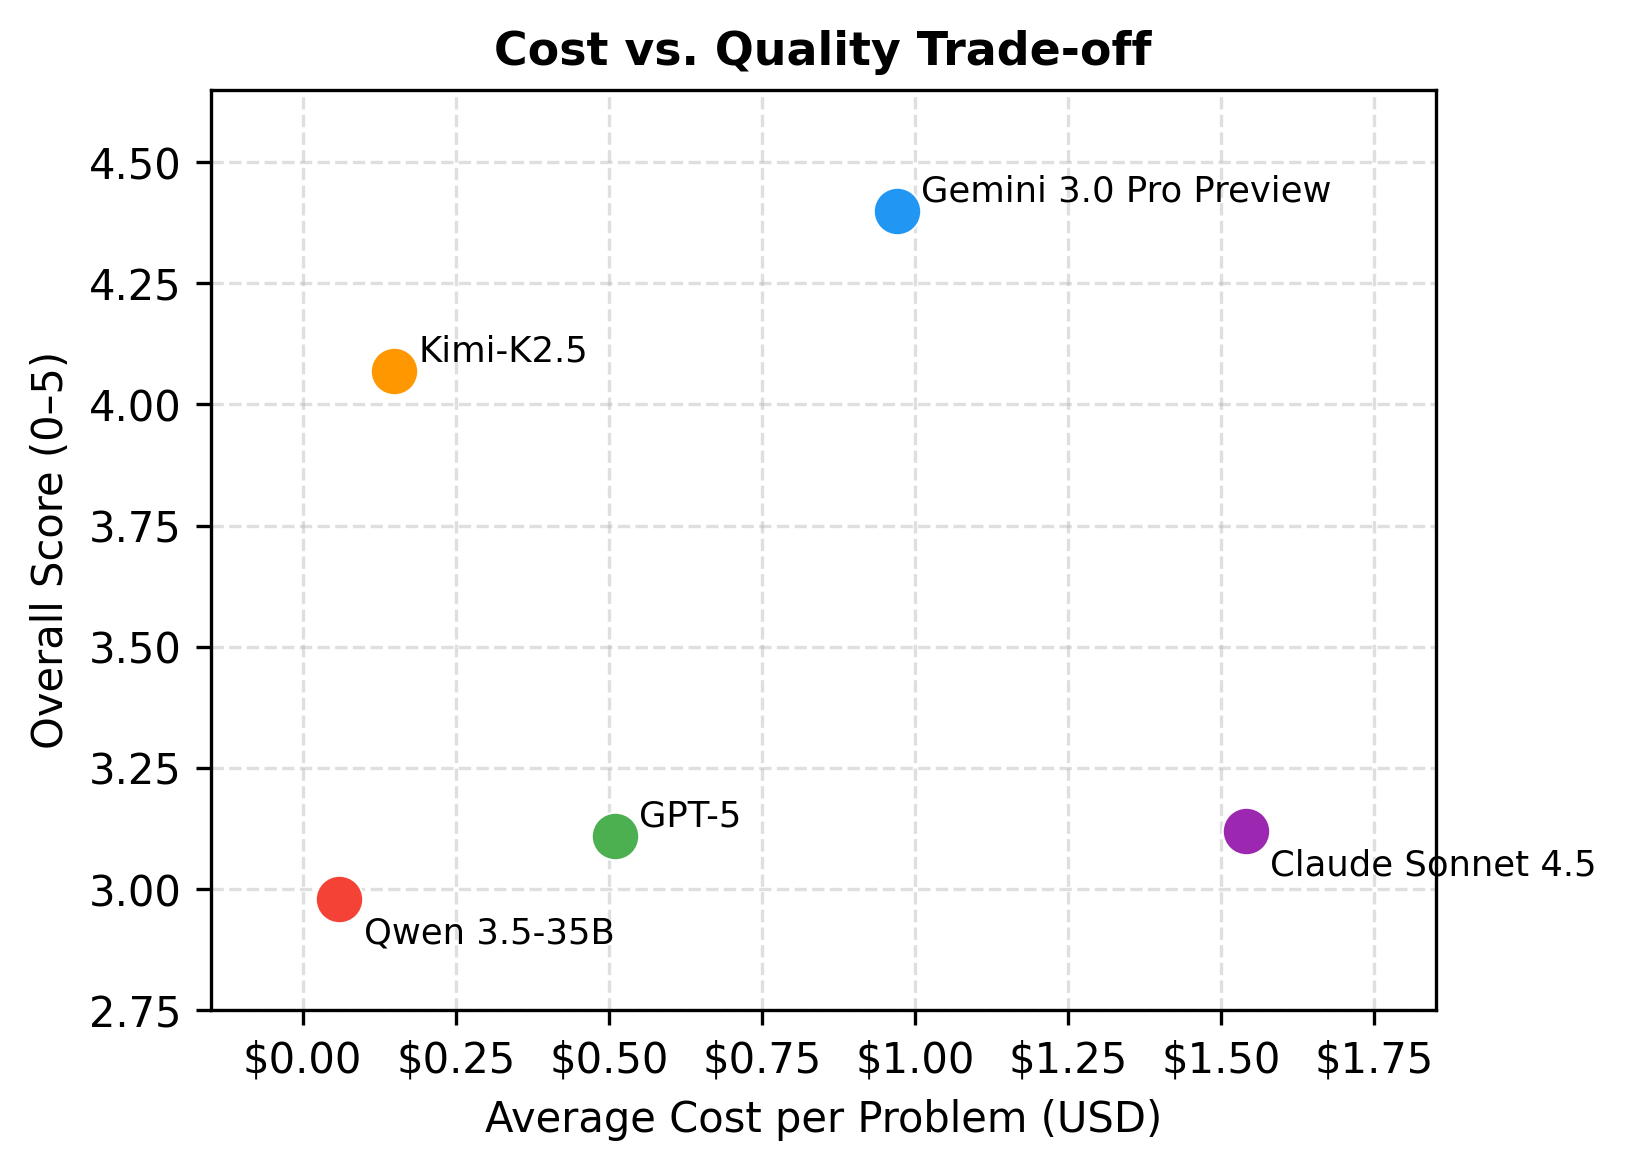
\includegraphics[width=\columnwidth]{fig/fig_cost_quality.png}
  \caption{Cost vs.\ quality trade-off across five models. X-axis: average cost per problem (USD); Y-axis: overall score (0--5). Kimi-K2.5 offers the best cost-efficiency, achieving 4.07 at \$0.15/problem.}
  \label{fig:cost-quality}
\end{figure}

\section{Conclusion}

We introduced EduIllustrate, the first comprehensive system and benchmark for generating and evaluating diagram-rich K-12 STEM problem explanations. Our four-stage pipeline decomposes multimodal content creation into structured outline generation, scene implementation planning, code generation with sequential Scene 1 anchoring, and document assembly, enabling frontier LLMs to produce geometrically accurate diagrams integrated with step-by-step textual reasoning. The benchmark comprises 118 problems spanning three grade levels and five subjects, evaluated through an 8-dimension rubric grounded in multimedia learning theory assessing both text quality and visual quality.

Evaluation of five state-of-the-art LLMs reveals that Gemini 3.0 Pro Preview achieves highest overall quality (4.40/5.0), while Kimi-K2.5 offers strong cost-effectiveness (4.07 score at \$0.15/problem, 10$\times$ cheaper than Gemini). Workflow ablation validates our sequential Scene 1 anchoring strategy, demonstrating 12\% improvement in visual consistency over fully parallel generation at 17.5\% lower cost. Human evaluation with 20 expert raters establishes strong human-AI agreement on objective dimensions (logical coherence: $\rho = 0.89$, diagram-problem alignment: $\rho = 0.83$), validating LLM-as-judge for scalable automated evaluation, while revealing limitations on subjective visual assessment (layout quality: $\rho = 0.39$, visual consistency: $\rho = 0.47$). Cost analysis shows generating explanations for complete K-12 curricula ranges from \$300-\$7,700 depending on model choice, far below typical textbook development costs (\$50K-\$200K), positioning automated content generation as economically viable for institutional deployment.

However, pedagogical effectiveness remains the weakest dimension across all models (2.54-3.91), indicating current LLMs produce \textit{correct} explanations more easily than \textit{pedagogically effective} explanations. This gap underscores the need for human expert review before classroom deployment and suggests LLMs augment rather than replace human educators. Future work should extend to video generation with temporal evaluation metrics, conduct classroom efficacy studies with learning outcome measures, expand to multilingual benchmarks covering diverse educational systems, and develop specialized pedagogical effectiveness models fine-tuned on expert-annotated explanations.

\section*{Limitations}

\textbf{Static Diagrams Only.} The pipeline generates static PNG images rather than animations. While static diagrams align with textbook pedagogy and Cognitive Load Theory research~\citep{ji2025eduvis} suggests animations can increase extraneous load for complex topics, extending to short educational videos (5-15 seconds) would enhance understanding of temporal processes. This requires developing temporal evaluation metrics beyond our 8-dimension rubric and validating effectiveness through eye-tracking studies.

\textbf{LLM-as-Judge Visual Assessment Limitations.} Weak human-AI agreement on visual dimensions (D5 Element Layout: $\rho = 0.39$, D6 Visual Consistency: $\rho = 0.47$) indicates current vision-language models struggle to assess layout quality and stylistic consistency reliably. Low inter-rater agreement among humans ($\alpha \approx 0.30$) suggests these constructs are ill-defined, requiring rubric refinement through exemplar diagrams for each score level or decomposition into objective binary checks (e.g., element overlap detection, color scheme extraction and comparison). Future work should explore specialized visual quality assessment models fine-tuned on human-annotated diagram datasets.

\textbf{Dataset Scope Constraints.} All 118 problems derive from Chinese K-12 curricula, limiting cross-cultural generalizability. Chemistry (8 problems) and biology (10 problems) constitute only 15\% of the benchmark due to dataset availability constraints. Expanding to 30-40 problems per subject and including problems from US Common Core, UK National Curriculum, and other educational systems would strengthen conclusions. Additionally, evaluation uses Gemini 3.0 Pro Preview (optimized for English) as judge model---replication with Chinese-specific judge models could reveal language-dependent evaluation bias.

\textbf{Technical Implementation Constraints.} The pipeline is tightly coupled to Manim, limiting generalizability to other frameworks (TikZ, matplotlib, SVG). Extending to target-agnostic intermediate representations as proposed by~\citet{kumar2025diagramir} would improve flexibility. The 8-dimension rubric evaluates multiple pedagogical facets through single scores (e.g., D4 conflates language complexity, scaffolding strategy, and misconception anticipation), requiring decomposition for finer-grained analysis. Finally, pedagogical effectiveness evaluation relies on expert judgment rather than learning outcomes---classroom efficacy studies with pre/post-test designs would provide ground truth for educational impact.

\section*{Acknowledgments}

We thank the 20 expert raters (15 STEM graduate students and 5 education doctoral students) for their meticulous human evaluation work. We acknowledge support from [funding agency] under grant [number].






\bibliography{custom}

\appendix

\section{Benchmark Problem Details}
\label{sec:benchmark-details}

Table~\ref{tab:benchmark-full} lists the complete knowledge point coverage of the 118 benchmark problems, organized by grade level and subject.

\begin{table*}[t]
\centering
\small
\begin{tabular}{llp{10cm}}
\hline
\textbf{Level} & \textbf{Subject} & \textbf{Knowledge Points} \\
\hline
\multirow{5}{*}{High School}
 & Biology (5)
 & Law of independent assortment; PCR amplification of DNA; Variants of 9:3:3:1 and 1:1:1:1 ratios; Sex-linked inheritance; Determination of gene locus on chromosomes \\
\cline{2-3}
 & Chemistry (5)
 & Galvanic and electrolytic cell principles (×2); Crystal structure and properties; Chemical equilibrium (equivalent equilibrium) \\
\cline{2-3}
 & Geography (5)
 & Earth and maps; General characteristics of Earth's motion \\
\cline{2-3}
 & Mathematics (20)
 & Proportional segments related to circles; Hyperbola properties; Proposition truth and plane-plane relations; Proposition truth and pyramid structure; Inscribed polygon properties; Tangent line proof and proportional segments; Common features of conic sections; Plane-plane perpendicularity; Parabola properties; Limits of sequences; Ellipse properties; Law of sines; Sphere volume and surface area; Area/volume from three-view drawings; Spatial line-line relations; Arithmetic sequences; Spatial vectors and sphere; (some topics unlabeled) \\
\cline{2-3}
 & Physics (20)
 & Concurrent force equilibrium and electric field strength; Work-energy theorem and projectile motion; Work-energy theorem and charged particle in uniform electric field; Work-energy theorem and mechanical energy conservation; Conservation of momentum; Momentum, mechanical energy, and energy conservation; EMF from conductor motion and Joule's law (×3, various combinations); Charged particle in uniform electric field (×2, with work-energy theorem); Coulomb's law and Newton's second law; Mechanical energy conservation and projectile; Ideal gas law and enclosed gas pressure; SHM amplitude/period/frequency, vertical projection, Hooke's law; Energy conservation, steady current, and force equilibrium \\
\hline
\multirow{5}{*}{Middle School}
 & Biology (5)
 & DNA replication/transcription/translation calculations; Complete and incomplete metamorphosis in insects; Urinary system and urine formation \\
\cline{2-3}
 & Chemistry (3)
 & Molecules, atoms, ions, elements and matter; Molecular definition and acid-base indicators; Chemical inference, decomposition and displacement reactions \\
\cline{2-3}
 & Geography (5)
 & Latitude and longitude; Principles of day length variation and seasons; Determining direction and location using coordinate grids (×3) \\
\cline{2-3}
 & Mathematics (20)
 & Linear function applications; Triangle angle sum and exterior angles; Triangle angle sum and rotation; Circumscribed circle and circumcenter; Quadratic/linear function graphs and coefficients; Triangle congruence (SAS) and Pythagorean theorem; 3D solid nets; Similar triangles (judgment and properties); Geometric solid nets; Inequalities, linear and quadratic functions (comprehensive); 30$^\circ$ right triangle, inscribed angles, and diameter angles; Net folding; Proportional segments, midsegment, and 30$^\circ$ triangle; Rotation and area; Square properties and coordinates; Similar triangles and equilateral triangle; Fold transformations; Axial symmetry; Golden ratio and right triangle solving \\
\cline{2-3}
 & Physics (20)
 & Force balance and pulley systems; Diagnosing circuit faults with ammeter/voltmeter; Force and motion; Pressure comparison, density, gravity vs.\ pressure; Balanced forces and kinetic/potential energy; Spring force meter; Friction force; Lever equilibrium (×2, including minimum force); Ohm's law and electromagnet factors; Ohm's law applications; Pulley rope tension, work, and power; Ammeter usage; Three circuit states; Dynamic circuit analysis (×2, with power); Magnetic pole interactions and Ampere's right-hand rule; Archimedes' principle and force balance (×2) \\
\hline
Elementary & Mathematics (10)
 & Three-view and net diagrams; Observing 3D shapes from different views; Shape composition; Position and direction; Rotation and coordinate position; Perimeter of composite plane figures; Overlapping problems; Cube/cuboid nets and folding \\
\hline
\end{tabular}
\caption{Complete knowledge point coverage of the 118 EduIllustrate benchmark problems. Numbers in parentheses indicate problem count per subject-level combination. Some high school mathematics problems have unlabeled knowledge points in the original K12-Vista dataset.}
\label{tab:benchmark-full}
\end{table*}

\section{Visual Consistency Case Study}
\label{sec:case-study}

To illustrate the impact of our sequential Scene 1 anchoring strategy on visual consistency (D6), we present a side-by-side comparison of two explanations generated for the same high school mathematics problem (four-pyramid $P$-$ABCD$, finding $NC:NP$ given $MN \parallel$ plane $PAD$). Both explanations are generated by Gemini 3.0 Pro Preview: the top row uses our workflow (sequential Scene 1 planning + parallel Scenes 2--N conditioned on Scene 1's code), while the bottom row uses the all-parallel baseline (all scenes planned and generated independently).

\begin{figure*}[t]
  \centering
  \textbf{Ours (Sequential Anchoring) --- D6 = 4.42}\\[4pt]
  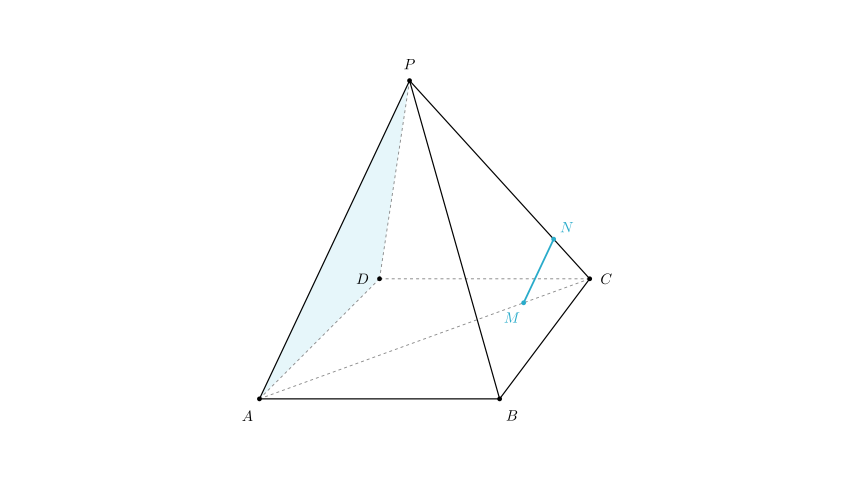
\includegraphics[width=0.32\textwidth]{fig/doc1_scene1.png}\hfill
  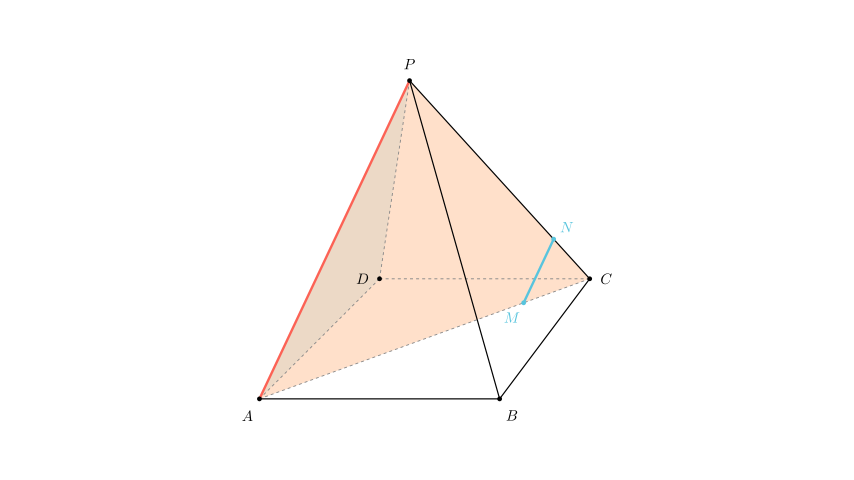
\includegraphics[width=0.32\textwidth]{fig/doc1_scene2.png}\hfill
  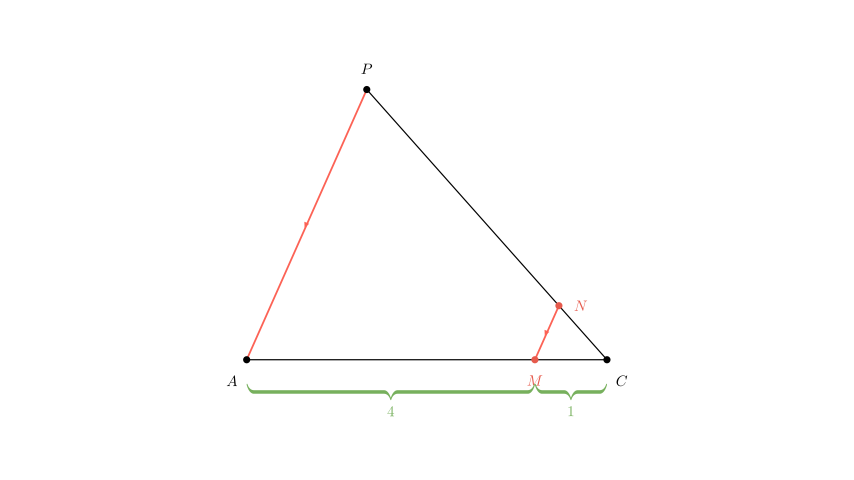
\includegraphics[width=0.32\textwidth]{fig/doc1_scene3.png}\\[10pt]
  \textbf{All-Parallel Baseline --- D6 = 3.89}\\[4pt]
  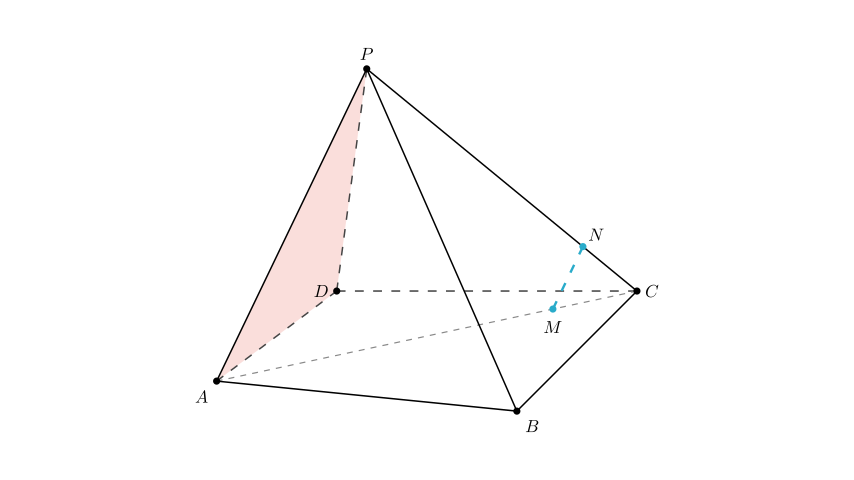
\includegraphics[width=0.32\textwidth]{fig/doc2_scene1.png}\hfill
  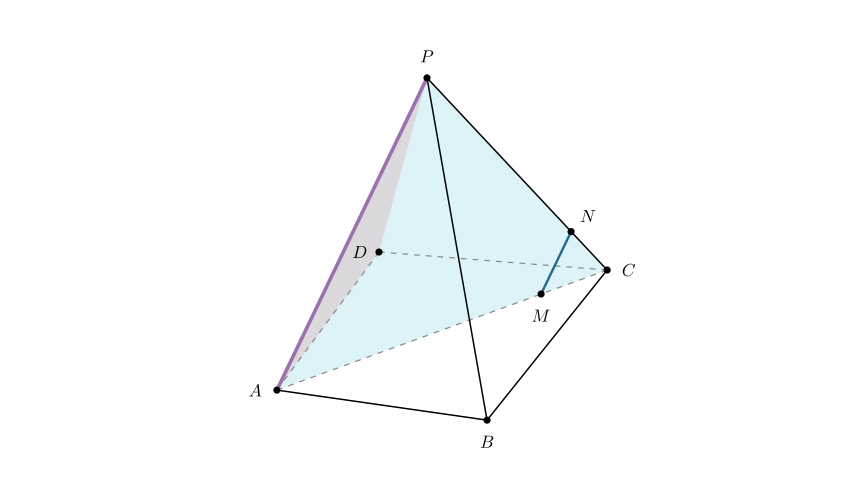
\includegraphics[width=0.32\textwidth]{fig/doc2_scene2.png}\hfill
  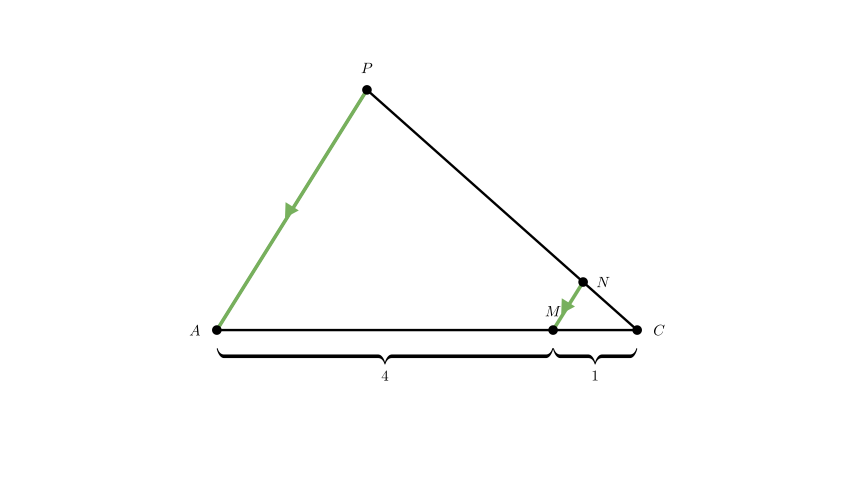
\includegraphics[width=0.32\textwidth]{fig/doc2_scene3.png}
  \caption{Visual consistency comparison between our sequential anchoring workflow (top) and the all-parallel baseline (bottom) on the same problem (four-pyramid $P$-$ABCD$). In our workflow, Scene 1 and Scene 2 render the identical pyramid structure---Scene 2 simply highlights the $PAC$ face on top of the same base diagram---maintaining full geometric and stylistic consistency. In the all-parallel baseline, the pyramid in Scene 1 and Scene 2 is drawn differently, breaking visual coherence and forcing the reader to reconcile two inconsistent representations of the same object.}
  \label{fig:case-study}
\end{figure*}

\section{A Gallery of Generated Explanations}
\label{sec:gallery}

We present representative high-quality and low-quality explanations generated by EduIllustrate to illustrate the range of outputs across different subjects and failure modes. Each entry shows the problem statement, key solution steps, and the corresponding rendered diagrams.

\subsection*{High-Quality Explanations}

\noindent Example 1: Middle School Physics (Circuit Analysis)

\begin{figure*}[h]
\centering
\begin{minipage}[t]{0.48\textwidth}
\scriptsize
\textbf{Problem:} The circuit is shown. Which analysis is incorrect? (A) After S is closed, the circuit short-circuits. (B) After S is closed, $L_1$ and $L_2$ are in parallel and both light up. (C) Removing wire $b$ makes $L_1$ and $L_2$ series-connected. (D) Moving wire $M$ from B to A makes $L_1$ and $L_2$ parallel.\\[4pt]
\textbf{Approach:} Trace current paths from the positive terminal to determine circuit topology under each scenario, then evaluate each option.\\[4pt]
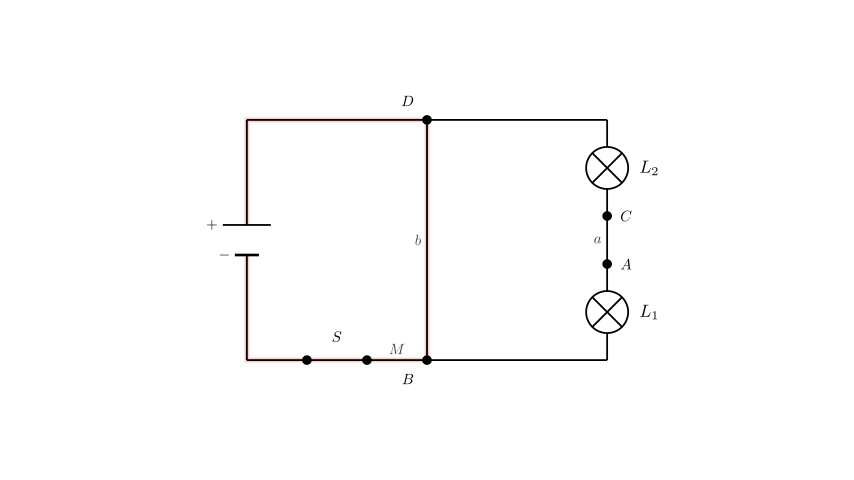
\includegraphics[width=\linewidth]{fig/doc_problem_4_gemini-3-pro-preview_scene1.png}\\[2pt]
\scriptsize\textit{Scene 1: Original circuit diagram with current path analysis. Wire $b$ short-circuits the bulbs, creating a zero-resistance path.}
\end{minipage}\hfill
\begin{minipage}[t]{0.48\textwidth}
\scriptsize
\textbf{Step 2:} Removing wire $b$ forces current through $L_2 \to L_1$ sequentially---series connection confirmed.\\[4pt]
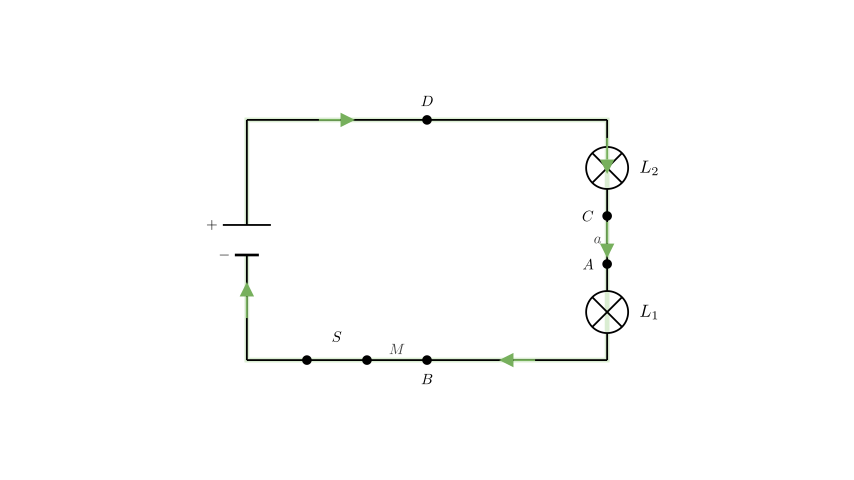
\includegraphics[width=\linewidth]{fig/doc_problem_4_gemini-3-pro-preview_scene2.png}\\[2pt]
\scriptsize\textit{Scene 2: Modified circuit with wire $b$ removed. Single current path through both bulbs in series.}\\[4pt]
\textbf{Step 3:} Moving wire $M$ from B to A creates two independent paths. Both bulbs connect between the same high/low potential nodes---parallel connection.\\[4pt]
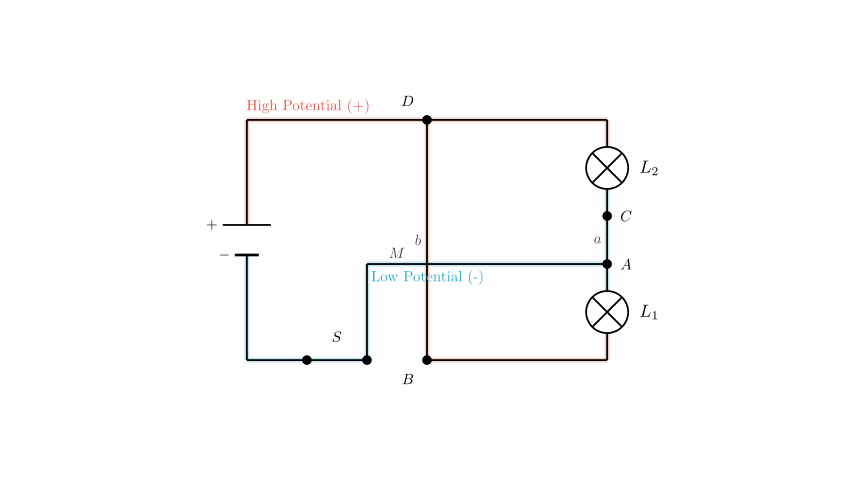
\includegraphics[width=\linewidth]{fig/doc_problem_4_gemini-3-pro-preview_scene3.png}\\[2pt]
\scriptsize\textit{Scene 3: Circuit with wire $M$ moved to A. Both bulbs span identical potential difference---parallel.}\\[4pt]
\textbf{Answer: B} (bulbs do not light up; short circuit prevents current through loads).
\end{minipage}
\caption*{\textbf{High-quality example 1.} Diagrams consistently use the same circuit drawing conventions across all three scenes. Each scene incrementally modifies the previous one, supporting step-by-step reasoning.}
\end{figure*}

\noindent Example 2: Middle School Biology (DNA Structure \& Replication)

\begin{figure*}[h]
\centering
\begin{minipage}[t]{0.48\textwidth}
\scriptsize
\textbf{Problem:} A $^{15}$N-labeled eukaryotic gene has Cytosine (C) accounting for 30\% of all bases. Which statement is correct? (A) Helicase acts on sites \textcircled{1} and \textcircled{2}. (B) In one strand, (C+G)/(A+T) = 3:2. (C) After $T\to A$ mutation at site \textcircled{1}, after $n$ replications the mutant gene is 1/4. (D) After 3 replications in $^{14}$N medium, DNA with $^{14}$N is 3/4.\\[4pt]
\textbf{Approach:} Identify bond types at sites \textcircled{1} and \textcircled{2}; apply Chargaff's rules; apply semi-conservative replication.\\[4pt]
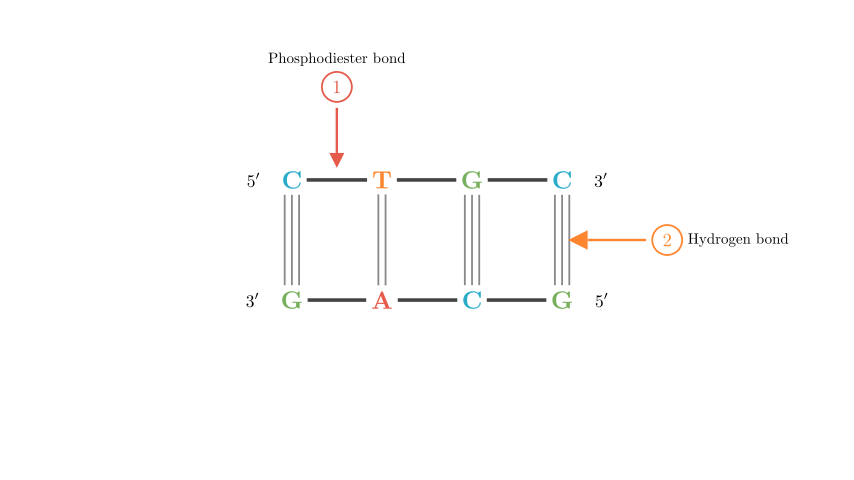
\includegraphics[width=\linewidth]{fig/doc_problem_46_gemini-3-pro-preview_scene1.png}\\[2pt]
\scriptsize\textit{Scene 1: DNA double helix with sites \textcircled{1} (hydrogen bonds between bases) and \textcircled{2} (phosphodiester bonds in backbone) clearly labeled.}
\end{minipage}\hfill
\begin{minipage}[t]{0.48\textwidth}
\scriptsize
\textbf{Step 2:} Chargaff's rules: C=G=30\%, so A=T=20\%. Within one strand, C+G=60\%, A+T=40\%, giving ratio 3:2---Statement B is correct.\\[4pt]
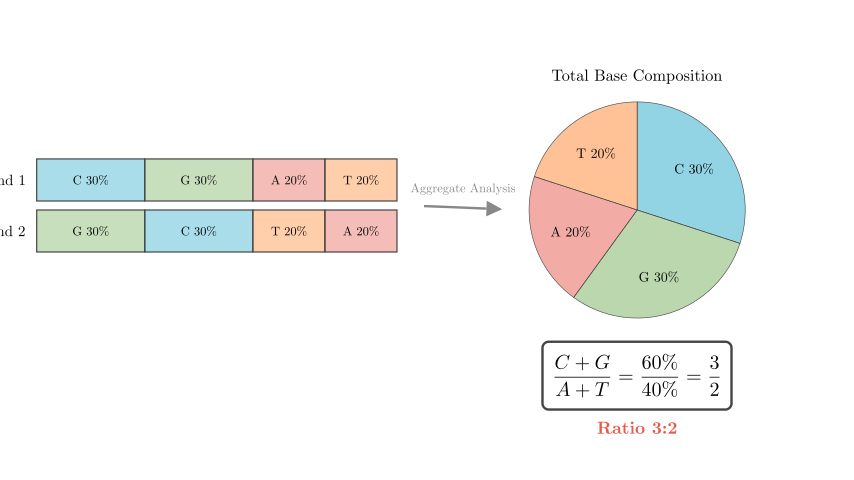
\includegraphics[width=\linewidth]{fig/doc_problem_46_gemini-3-pro-preview_scene2.png}\\[2pt]
\scriptsize\textit{Scene 2: Base composition diagram showing C/G/A/T proportions derived from Chargaff's rules.}\\[4pt]
\textbf{Step 3:} Semi-conservative replication after 3 rounds yields $2^3=8$ DNA molecules; all 8 contain $^{14}$N (since new strands use $^{14}$N); 2 of 8 also retain $^{15}$N. So $^{14}$N proportion = 8/8 = 100\%, not 3/4---Statement D is wrong.\\[4pt]
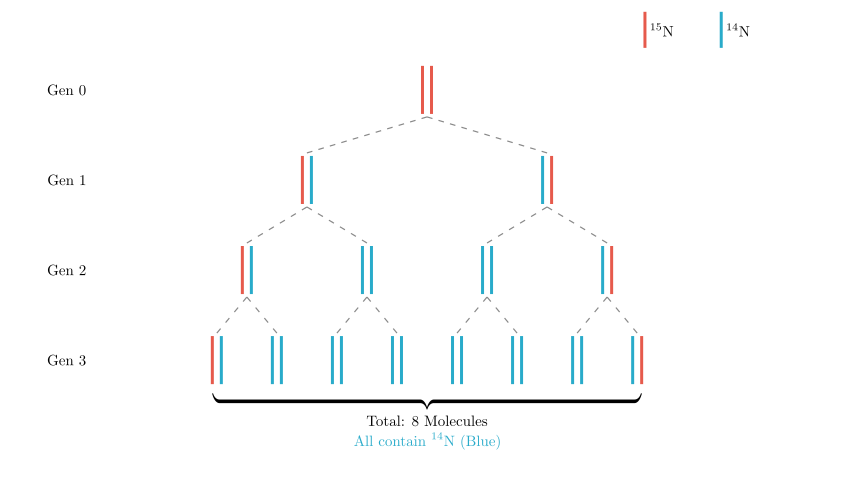
\includegraphics[width=\linewidth]{fig/doc_problem_46_gemini-3-pro-preview_scene3.png}\\[2pt]
\scriptsize\textit{Scene 3: Semi-conservative replication tree after 3 rounds, showing isotope distribution across 8 daughter molecules.}\\[4pt]
\textbf{Answer: B.}
\end{minipage}
\caption*{\textbf{High-quality example 2.} Diagrams use consistent color coding (blue for $^{15}$N strands, orange for $^{14}$N strands) across all scenes, with each scene building directly on the previous one.}
\end{figure*}

\noindent Example 3: High School Math (Infinite Geometric Series, Inscribed Circles)

\begin{figure*}[h]
\centering
\begin{minipage}[t]{0.48\textwidth}
\scriptsize
\textbf{Problem:} A regular hexagon is inscribed in a circle of radius 1 m. Its inscribed circle is drawn, inside which another regular hexagon is inscribed, and so on infinitely. Find the sum $S$ of the areas of all circles.\\[4pt]
\textbf{Approach:} Find the ratio between successive circle radii using the apothem of a regular hexagon, identify the geometric series common ratio, then apply the infinite sum formula.\\[4pt]
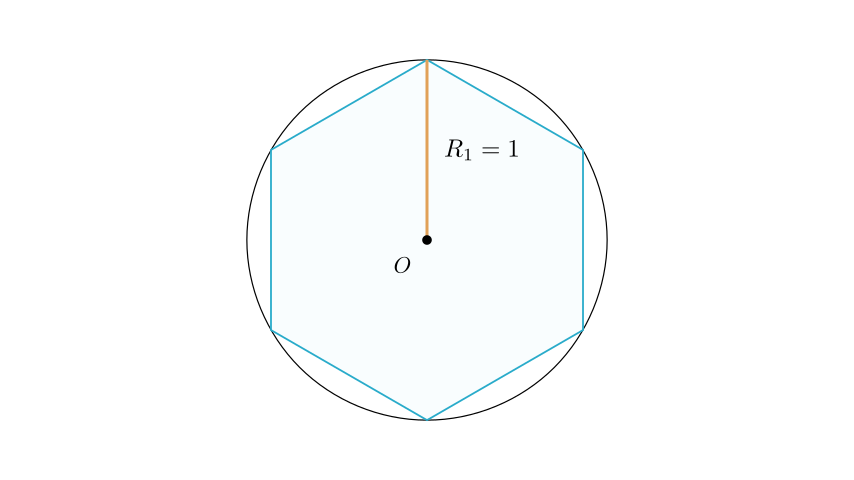
\includegraphics[width=\linewidth]{fig/doc_problem_56_gemini-3-pro-preview_scene1.png}\\[2pt]
\scriptsize\textit{Scene 1: First circle ($R_1=1$) with inscribed hexagon and its apothem shown. The apothem equals $\frac{\sqrt{3}}{2}R_1$, giving $R_2=\frac{\sqrt{3}}{2}$.}
\end{minipage}\hfill
\begin{minipage}[t]{0.48\textwidth}
\scriptsize
\textbf{Step 2:} Area ratio $= \left(\frac{R_2}{R_1}\right)^2 = \frac{3}{4}$. The areas form a geometric series with first term $\pi$ and common ratio $\frac{3}{4}$.\\[4pt]
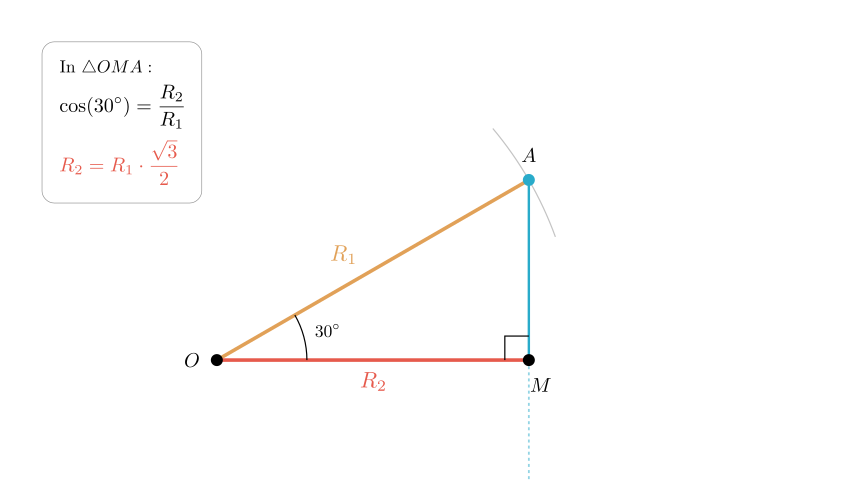
\includegraphics[width=\linewidth]{fig/doc_problem_56_gemini-3-pro-preview_scene2.png}\\[2pt]
\scriptsize\textit{Scene 2: First two circles and hexagons overlaid, illustrating the scaling relationship.}\\[4pt]
\textbf{Step 3:} $S = \frac{\pi}{1 - \frac{3}{4}} = 4\pi$ m$^2$.\\[4pt]
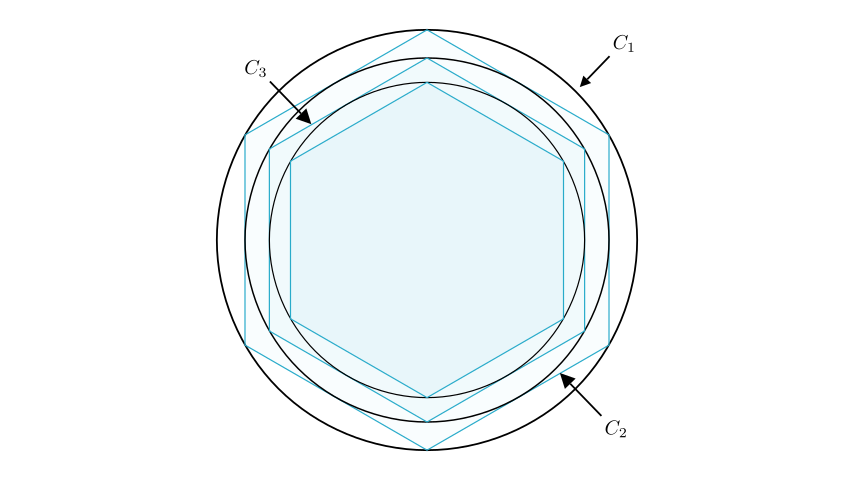
\includegraphics[width=\linewidth]{fig/doc_problem_56_gemini-3-pro-preview_scene3.png}\\[2pt]
\scriptsize\textit{Scene 3: Infinite nesting visualized with converging circles and hexagons.}\\[4pt]
\textbf{Answer: $S = 4\pi$ m$^2$.}
\end{minipage}
\caption*{\textbf{High-quality example 3.} Each scene builds progressively on the previous geometric construction, with consistent styling and annotations.}
\end{figure*}

\noindent Example 4: High School Math (Solid Geometry, Perpendicular Planes)

\begin{figure*}[h]
\centering
\begin{minipage}[t]{0.48\textwidth}
\scriptsize
\textbf{Problem:} In quadrangular pyramid $P$-$ABCD$, $PA \perp$ base $ABCD$, all base edges are equal (rhombus). $M$ is a moving point on $PC$. State a condition on $M$ such that plane $MBD \perp$ plane $PCD$.\\[4pt]
\textbf{Approach:} Use the plane-perpendicularity theorem: find a line in plane $MBD$ perpendicular to plane $PCD$. Show $BD \perp PC$ using the rhombus diagonal and $PA \perp$ base properties, then determine where $MBD$ must intersect $PCD$.\\[4pt]
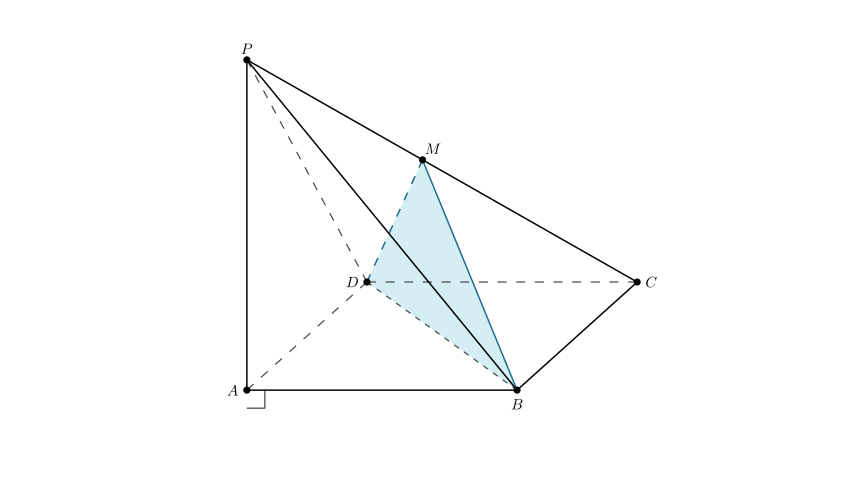
\includegraphics[width=\linewidth]{fig/doc_problem_70_gemini-3-pro-preview_scene1.png}\\[2pt]
\scriptsize\textit{Scene 1: Pyramid with rhombus base $ABCD$, $PA$ perpendicular to base, diagonal $BD$ highlighted.}
\end{minipage}\hfill
\begin{minipage}[t]{0.48\textwidth}
\scriptsize
\textbf{Step 2:} Since $ABCD$ is a rhombus, $AC \perp BD$. Since $PA \perp$ base, $PA \perp BD$. Thus $BD \perp$ plane $PAC$, hence $BD \perp PC$.\\[4pt]
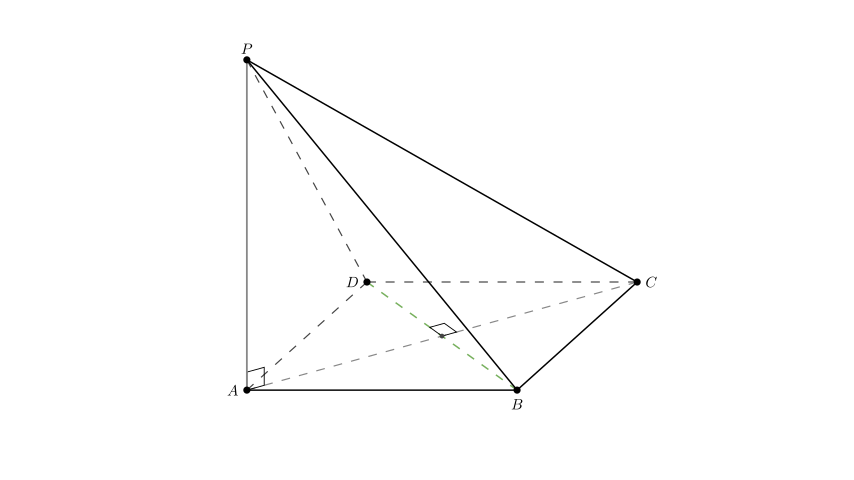
\includegraphics[width=\linewidth]{fig/doc_problem_70_gemini-3-pro-preview_scene2.png}\\[2pt]
\scriptsize\textit{Scene 2: Plane $PAC$ highlighted, showing $BD \perp$ plane $PAC$ and therefore $BD \perp PC$.}\\[4pt]
\textbf{Step 3:} $BD \perp PC$ and $BD \subset$ plane $MBD$; if $M$ is the foot of the altitude from $B$ to $PC$ (i.e., $MB \perp PC$), then $BD \perp$ plane $PCD$, giving plane $MBD \perp$ plane $PCD$.\\[4pt]
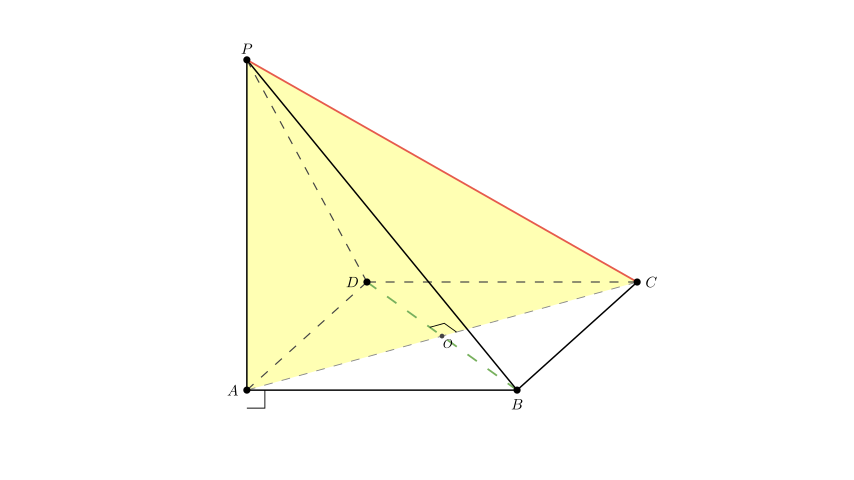
\includegraphics[width=\linewidth]{fig/doc_problem_70_gemini-3-pro-preview_scene3.png}\\[2pt]
\scriptsize\textit{Scene 3: Plane $MBD$ and plane $PCD$ shown with their intersection line, confirming perpendicularity condition.}\\[4pt]
\textbf{Answer: $MB \perp PC$ (i.e., $M$ is the foot of the perpendicular from $B$ to $PC$).}
\end{minipage}
\caption*{\textbf{High-quality example 4.} Three scenes incrementally reveal the geometric reasoning: base properties, perpendicularity proof, and final plane configuration.}
\end{figure*}

\noindent Example 5: Middle School Math (Quadratic Function Coefficients)

\begin{figure*}[h]
\centering
\begin{minipage}[t]{0.48\textwidth}
\scriptsize
\textbf{Problem:} The graph of $y=ax^2+bx+1$ is shown. Which quadrant does $y=ax+b$ \textit{not} pass through?\\
A. First \quad B. Second \quad C. Third \quad D. Fourth\\[4pt]
\textbf{Approach:} Read signs of $a$ and $b$ from the parabola (opening direction, axis of symmetry position), then determine the linear function's slope and intercept to identify the missing quadrant.\\[4pt]
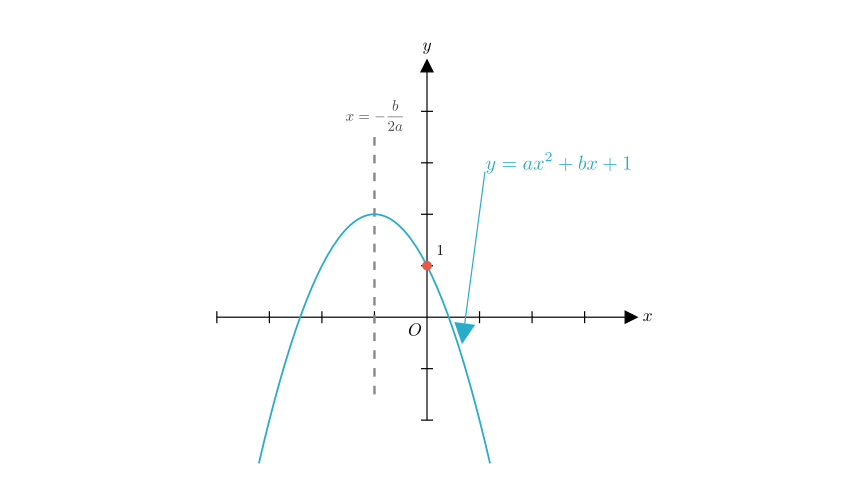
\includegraphics[width=\linewidth]{fig/doc_problem_97_gemini-3-pro-preview_scene1.png}\\[2pt]
\scriptsize\textit{Scene 1: Parabola opens downward ($a<0$), axis of symmetry at $x<0$, so $-b/(2a)<0 \Rightarrow b<0$.}
\end{minipage}\hfill
\begin{minipage}[t]{0.48\textwidth}
\scriptsize
\textbf{Step 2:} For $y=ax+b$: slope $a<0$ (decreasing), $y$-intercept $b<0$. A decreasing line with negative intercept passes through Quadrants II, III, IV---it does \textit{not} pass through Quadrant I.\\[4pt]
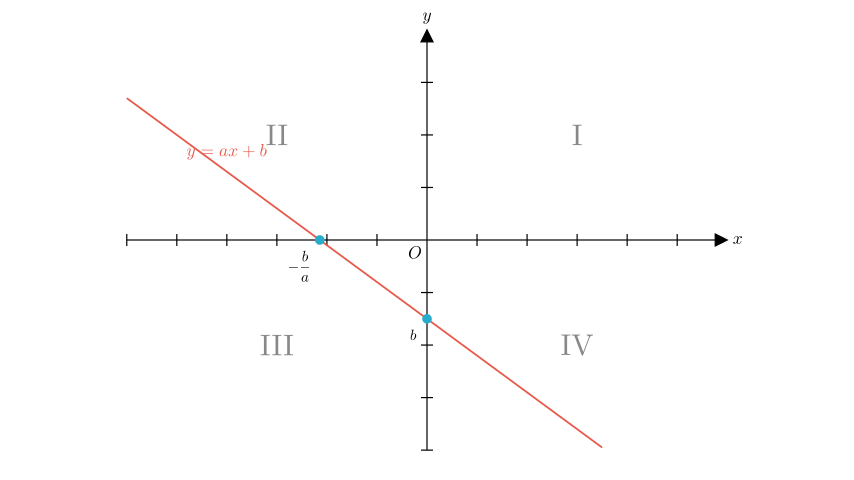
\includegraphics[width=\linewidth]{fig/doc_problem_97_gemini-3-pro-preview_scene2.png}\\[2pt]
\scriptsize\textit{Scene 2: Linear function $y=ax+b$ plotted with $a<0$, $b<0$, passing through Q2, Q3, Q4 only.}\\[4pt]
\textbf{Answer: A (First quadrant).}
\end{minipage}
\caption*{\textbf{High-quality example 5.} The parabola and linear function are rendered with consistent axis styles and color coding, with the missing quadrant clearly shaded.}
\end{figure*}

\noindent Example 6: Middle School Math (Square and Rhombus, Shaded Area)

\begin{figure*}[h]
\centering
\begin{minipage}[t]{0.48\textwidth}
\scriptsize
\textbf{Problem:} Square $ABCD$ has area 25; rhombus $PQCB$ has area 20. Find the area of the shaded region.\\
A. 11 \quad B. 6.5 \quad C. 7 \quad D. 7.5\\[4pt]
\textbf{Approach:} Determine side lengths from given areas; use the subtraction method to express the shaded area as the square minus an unshaded triangular region formed by the overlap of the square and rhombus.\\[4pt]
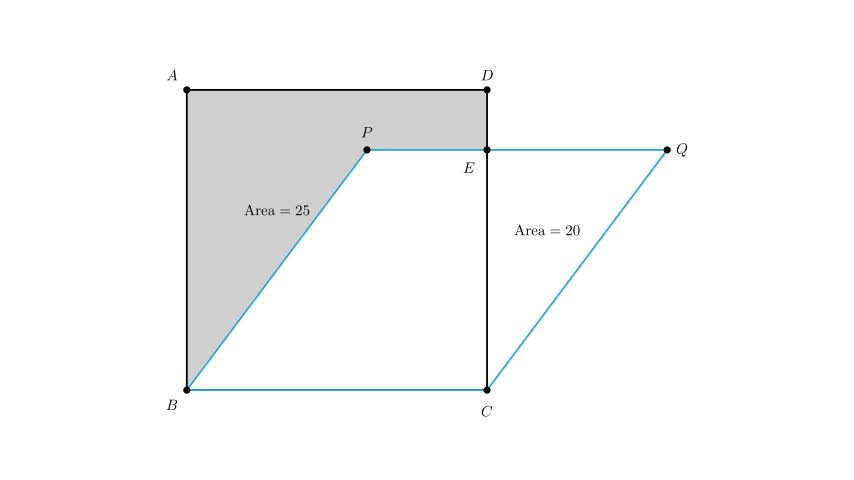
\includegraphics[width=\linewidth]{fig/doc_problem_103_gemini-3-pro-preview_scene1.png}\\[2pt]
\scriptsize\textit{Scene 1: Square $ABCD$ (side=5) and rhombus $PQCB$ overlaid; the shaded region and the unshaded overlap region clearly distinguished by color.}
\end{minipage}\hfill
\begin{minipage}[t]{0.48\textwidth}
\scriptsize
\textbf{Step 2:} Side of square = 5. Height of rhombus = area/base = 20/5 = 4. The unshaded region inside the square is a right triangle with legs 5 and $5-4=1$; its area = $\frac{1}{2}\times5\times1=2.5$. Shaded area $= 25 - 2\times2.5 \times \ldots$ (subtraction applied per configuration).\\[4pt]
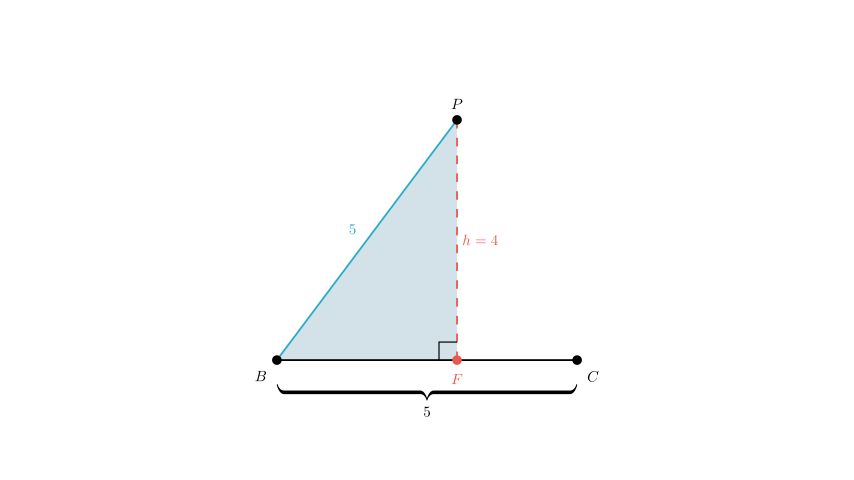
\includegraphics[width=\linewidth]{fig/doc_problem_103_gemini-3-pro-preview_scene2.png}\\[2pt]
\scriptsize\textit{Scene 2: Decomposition of the unshaded region into computable triangles.}\\[4pt]
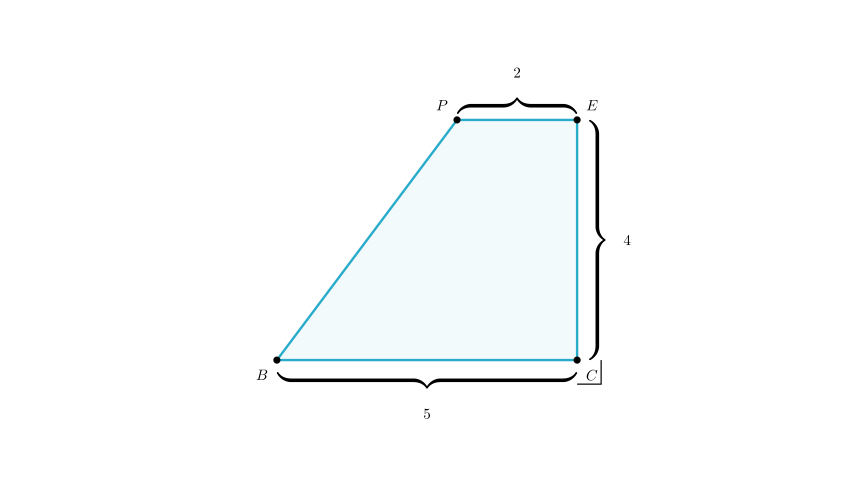
\includegraphics[width=\linewidth]{fig/doc_problem_103_gemini-3-pro-preview_scene3.png}\\[2pt]
\scriptsize\textit{Scene 3: Final shaded region highlighted with computed area.}\\[4pt]
\textbf{Answer: D (7.5).}
\end{minipage}
\caption*{\textbf{High-quality example 6.} Consistent color scheme across scenes: the square in blue, rhombus in orange, shaded region in green. Each scene progressively focuses on the region of interest.}
\end{figure*}

\subsection*{Low-Quality Explanations}

\noindent Example 7: Elementary Math (Cube Net Folding) --- Wrong Final Answer

\begin{figure*}[h]
\centering
\begin{minipage}[t]{0.48\textwidth}
\scriptsize
\textbf{Problem:} Xiaoxiao made a cubic gift box where opposite faces share the same pattern ($\star$, $\heartsuit$, $\odot$). Which net (A/B/C/D) folds into this cube?\\[4pt]
\textbf{Approach:} Apply opposite-face pairing rule for cross-type nets: positions (1,3), (2,4), and (top, bottom) are opposite pairs.\\[4pt]
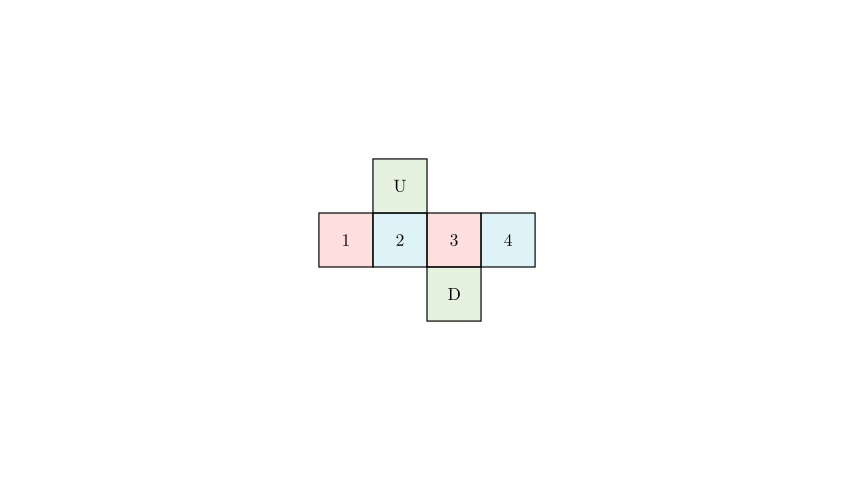
\includegraphics[width=\linewidth]{fig/doc_problem_40_gpt-5_scene1.png}\\[2pt]
\scriptsize\textit{Scene 1: Cross-type net with positions labeled and opposite-pair rule illustrated.}
\end{minipage}\hfill
\begin{minipage}[t]{0.48\textwidth}
\scriptsize
\textbf{Step 2:} Tests each option by mapping symbols to opposite-pair positions. Concludes that option C satisfies the constraint.\\[4pt]
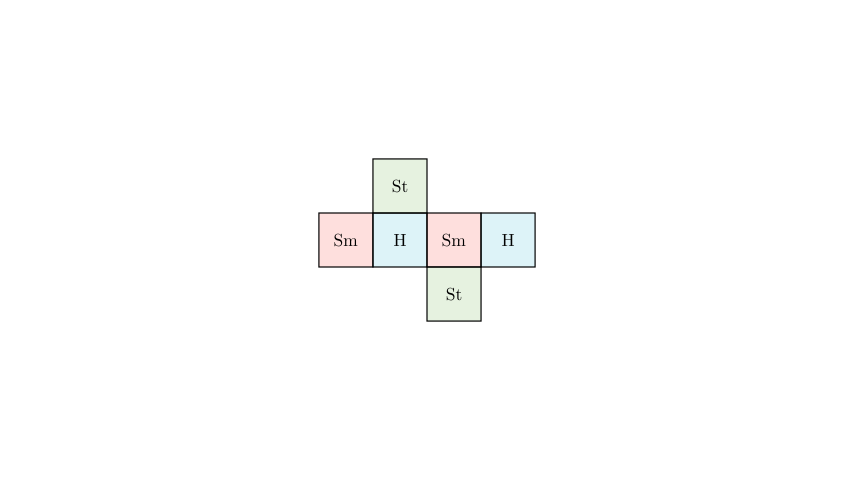
\includegraphics[width=\linewidth]{fig/doc_problem_40_gpt-5_scene2.png}\\[2pt]
\scriptsize\textit{Scene 2: Net options annotated with opposite-face verification.}\\[6pt]
\textbf{Final Answer: C} \hspace{4pt} \textcolor{red}{$\times$ \textbf{Gold answer: A}}\\[4pt]
\textbf{Failure mode (D1):} The reasoning process applies the opposite-face pairing rule correctly in principle, but misidentifies the symbol placement in option A vs.\ C during the mapping step, leading to an incorrect final answer.
\end{minipage}
\caption*{\textbf{Low-quality example 7 (D1 failure).} The model's final answer (C) contradicts the gold standard answer (A). Despite a structured approach, an error in reading the net topology causes the incorrect conclusion.}
\end{figure*}

\noindent Example 8: Middle School Math (Isosceles Triangle) --- Diagram Inconsistent with Problem

\begin{figure*}[h]
\centering
\begin{minipage}[t]{0.48\textwidth}
\scriptsize
\textbf{Problem:} In $\triangle ABC$, $AB=AC=4$, $\angle C=72^\circ$. Point $D$ is the midpoint of $AB$; point $E$ lies on $AC$; $DE \perp AB$. Find $\cos A$.\\
Options: A. $\frac{\sqrt{5}-1}{2}$ \quad B. $\frac{\sqrt{5}-1}{4}$ \quad C. $\frac{\sqrt{5}+1}{4}$ \quad D. $\frac{\sqrt{5}+1}{2}$\\[4pt]
\textbf{Approach:} Use isosceles triangle properties ($AB=AC \Rightarrow \angle B=\angle C=72^\circ$), compute $\angle A = 180^\circ-144^\circ=36^\circ$, then evaluate $\cos 36^\circ$.\\[4pt]
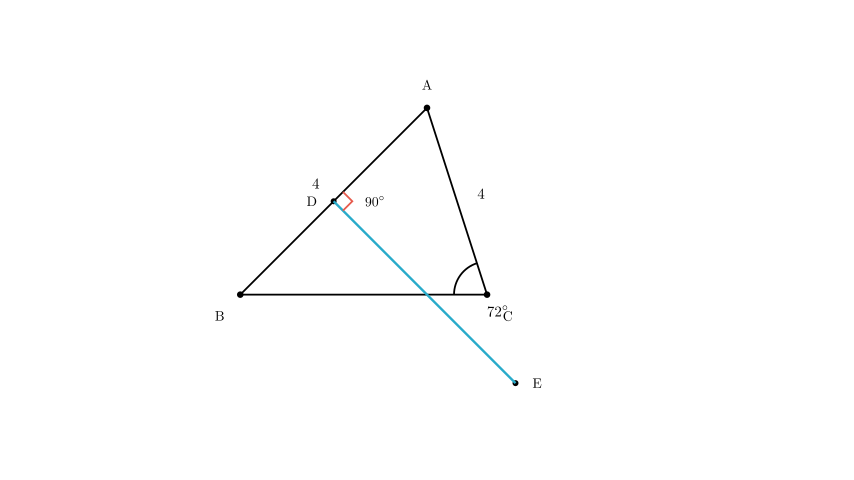
\includegraphics[width=\linewidth]{fig/doc_problem_111_gpt-5_scene1.png}\\[2pt]
\scriptsize\textit{Scene 1: \textcolor{red}{The diagram draws an acute scalene triangle with visibly unequal sides, violating the given $AB=AC$ constraint. The $72^\circ$ angles are not rendered at vertices B and C.}}
\end{minipage}\hfill
\begin{minipage}[t]{0.48\textwidth}
\scriptsize
\textbf{Step 2:} $\angle A + 72^\circ + 72^\circ = 180^\circ \Rightarrow \angle A = 36^\circ$.\\[4pt]
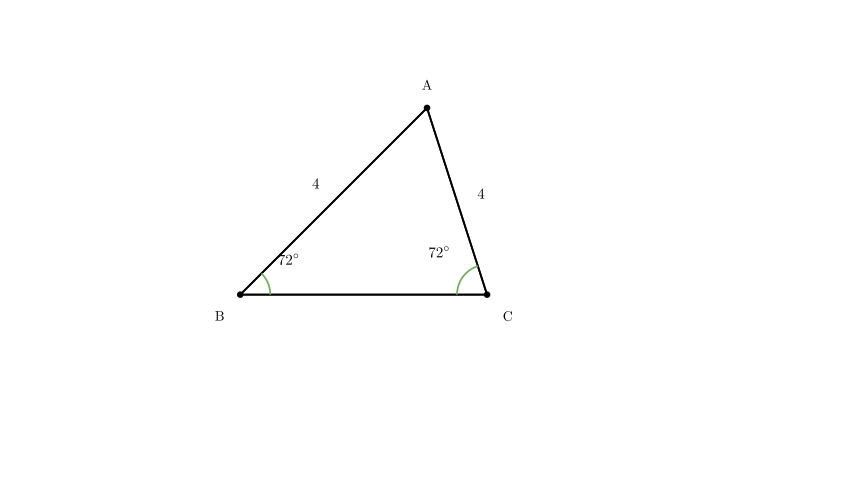
\includegraphics[width=\linewidth]{fig/doc_problem_111_gpt-5_scene2.png}\\[2pt]
\scriptsize\textit{Scene 2: \textcolor{red}{The highlighted triangle still shows inconsistent proportions. The isosceles constraint ($AB=AC$) is visually absent, making the diagram misleading.}}\\[4pt]
\textbf{Step 3:} $\cos 36^\circ = \frac{\sqrt{5}+1}{4}$\\[4pt]
\textbf{Final Answer: C} \hspace{4pt} \textcolor{green!60!black}{$\checkmark$} (textually correct)\\[4pt]
\textbf{Failure mode (D3):} Although the textual reasoning is correct, the rendered diagrams do not reflect the isosceles structure of the triangle---a fundamental geometric constraint of the problem. A student relying on the diagrams would form incorrect spatial intuitions.
\end{minipage}
\caption*{\textbf{Low-quality example 8 (D3 failure).} Diagrams fail to represent the isosceles triangle ($AB=AC$) and the $72^\circ$ base angles. Despite correct textual reasoning, the visual representations are geometrically inconsistent with the problem statement, undermining pedagogical effectiveness.}
\end{figure*}

\noindent Example 9: High School Physics (Gas Laws, Two Cylinders)--- Flawed Diagram

\begin{figure*}[h]
\centering
\begin{minipage}[t]{0.48\textwidth}
\scriptsize
\textbf{Problem:} Two connected vertical cylinders A (closed top, diameter $2d_B$, cross-section $4S$) and B (open top, diameter $d_B$, cross-section $S$), both height $H$. Piston $a$ in A is $H/4$ from the top; piston $b$ in B is at mid-height. $N_2$ fills below both pistons; $O_2$ fills above piston $a$. (1) Heat $N_2$ until piston $b$ reaches the top: find $N_2$ temperature. (2) Continue heating until piston $a$ rises $H/16$: find $O_2$ pressure.\\[4pt]
\textbf{Approach:} Stage I: $N_2$ expands at constant pressure $P_0$ (piston $b$ free); $O_2$ isothermal (constant volume). Stage II: $N_2$ volume in B fixed; $O_2$ compressed isothermally by Boyle's law.\\[4pt]
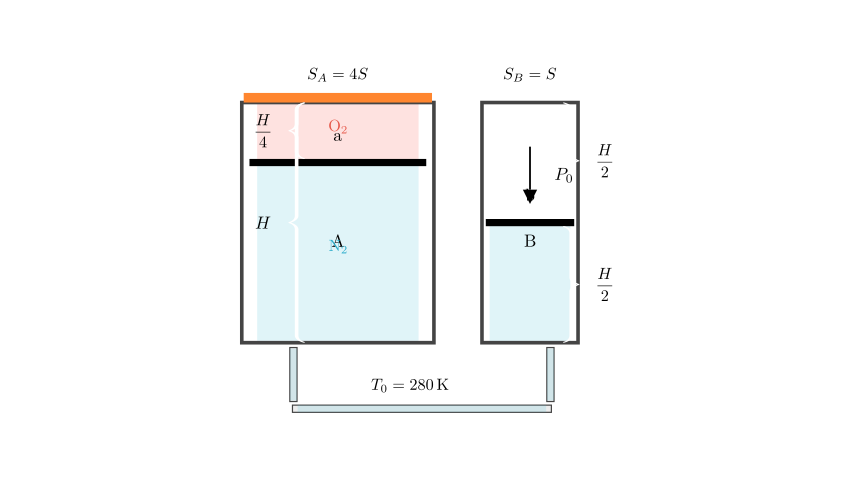
\includegraphics[width=\linewidth]{fig/doc_problem_85_gpt-5_scene1.png}\\[2pt]
\scriptsize\textit{Scene 1: \textcolor{red}{The height label below piston $a$ in cylinder A is marked $H$ instead of the correct $3H/4$, contradicting the given initial geometry and making the diagram inconsistent with the problem.}}
\end{minipage}\hfill
\begin{minipage}[t]{0.48\textwidth}
\scriptsize
\textbf{Step 2:} Stage I---$N_2$ volume changes from $V_{N0}=4S\cdot\frac{3H}{4}+S\cdot\frac{H}{2}=\frac{7SH}{2}$ to $V_{N1}=\frac{3SH}{4}\cdot4S+SH=4SH$. By $pV\propto T$: $T_1=T_0\cdot\frac{4SH}{7SH/2}=\frac{8}{7}T_0$.\\[4pt]
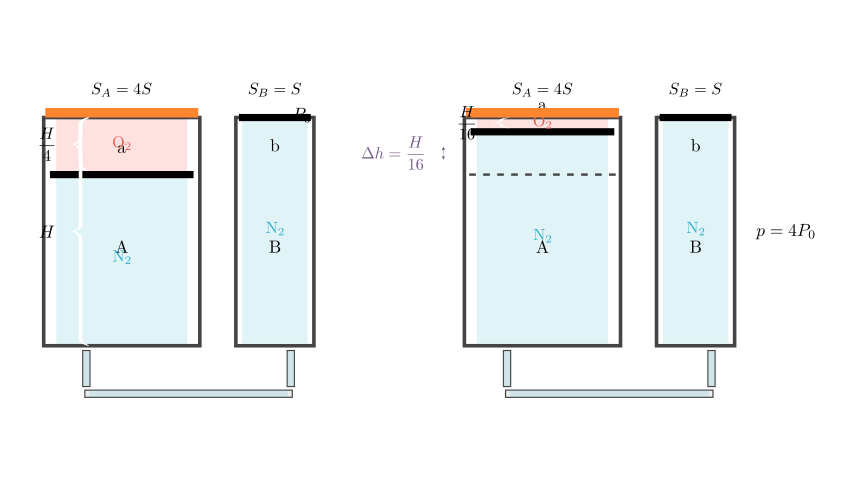
\includegraphics[width=\linewidth]{fig/doc_problem_85_gpt-5_scene2.png}\\[2pt]
\scriptsize\textit{Scene 2: \textcolor{red}{After piston $b$ reaches the top, the diagram still carries the incorrect label from Scene 1, propagating the error into Stage II.}}\\[4pt]
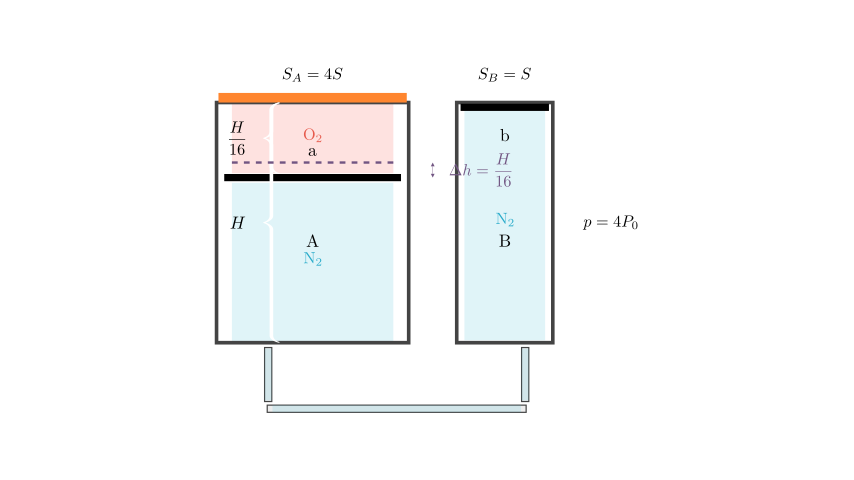
\includegraphics[width=\linewidth]{fig/doc_problem_85_gpt-5_scene3.png}\\[2pt]
\scriptsize\textit{Scene 3: Stage II diagram showing piston $a$ risen by $H/16$; layout partially corrected but inconsistent with Scene 1.}\\[4pt]
\textbf{Failure mode (D5/D3):} The mislabeled height $H$ (should be $3H/4$) in Scene 1 violates the problem's geometric constraints. A student using the diagram to set up equations would obtain wrong initial volumes and incorrect answers.
\end{minipage}
\caption*{\textbf{Low-quality example 5 (D3/D5 failure).} A critical geometric parameter ($3H/4$, the nitrogen column height in cylinder A) is mislabeled as $H$ in Scene 1 and Scene 2. The textual solution is correct, but the diagram directly contradicts the problem setup.}
\end{figure*}

\noindent Example 10: Middle School Geography (Latitude/Longitude Reading) --- Flawed Diagram Reading and Reasoning

\begin{figure*}[h]
\centering
\begin{minipage}[t]{0.48\textwidth}
\scriptsize
\textbf{Problem:} From a polar-view diagram of Earth with latitude circles and longitude markings, determine which statement is correct: (A) Point A receives direct sunlight only once a year. (B) Point B may receive direct sunlight twice a year. (C) Point B is in the Southern Hemisphere. (D) A is in the Eastern Hemisphere, B is in the Western Hemisphere.\\[4pt]
\textbf{Key facts:} Direct sunlight occurs only between $23.5^\circ$S and $23.5^\circ$N. Points on the tropics receive it once; points inside receive it twice. Hemisphere boundaries: equator (N/S), 20$^\circ$W--160$^\circ$E (E/W).\\[4pt]
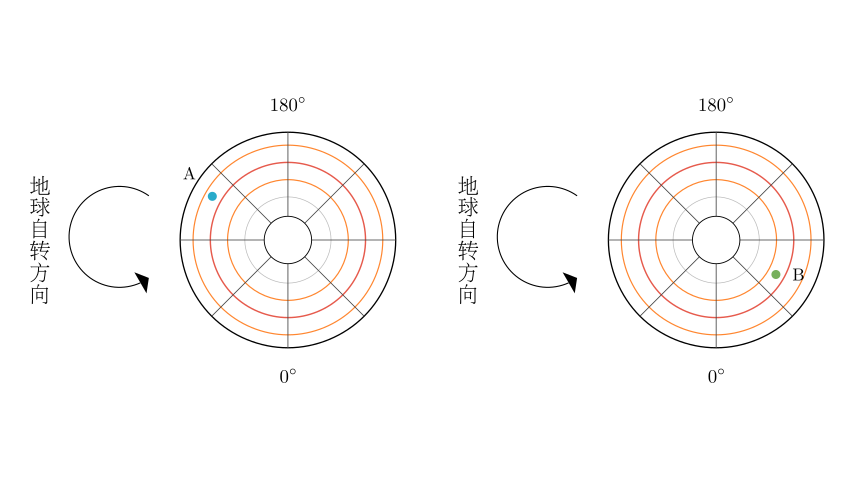
\includegraphics[width=\linewidth]{fig/doc_problem_114_gpt-5_scene1.png}\\[2pt]
\scriptsize\textit{Scene 1: Polar-view diagram. \textcolor{red}{The model incorrectly identifies point A as lying outside the tropics (mid-latitude), concluding A receives no direct sunlight---in fact, A is on the equator and receives direct sunlight twice a year.}}
\end{minipage}\hfill
\begin{minipage}[t]{0.48\textwidth}
\scriptsize
\textbf{Flawed reasoning:} The model misreads A as a mid-latitude point, eliminating option A with wrong logic. It then claims the diagram lacks explicit $0^\circ$/$180^\circ$ longitude markings to determine the E/W hemisphere---but the diagram does contain computable longitude references, making option D verifiable. The model eliminates options A, C, D through incorrect intermediate steps and selects B by elimination.\\[4pt]
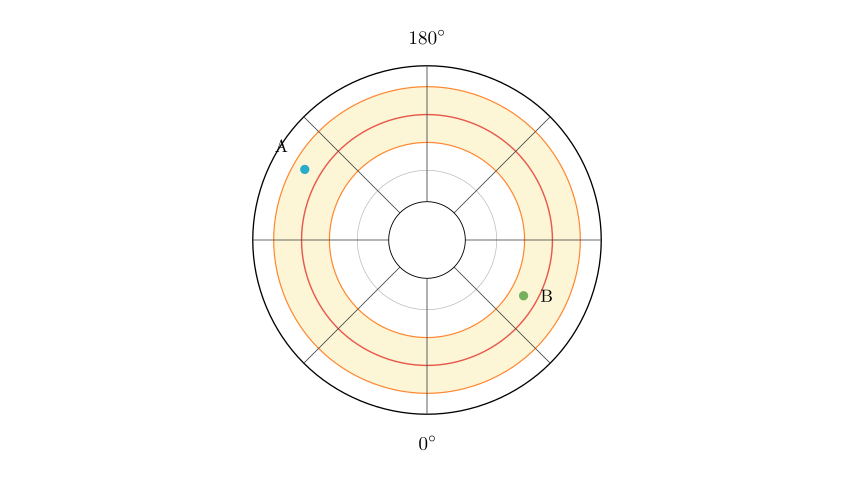
\includegraphics[width=\linewidth]{fig/doc_problem_114_gpt-5_scene2.png}\\[2pt]
\scriptsize\textit{Scene 2: Hemisphere analysis diagram. \textcolor{red}{The longitude reference lines drawn are inconsistent with the original diagram's markings, reflecting the model's failure to correctly read the given coordinate information.}}\\[4pt]
\textbf{Final Answer: B} \hspace{4pt} \textcolor{green!60!black}{$\checkmark$} (coincidentally correct)\\[4pt]
\textbf{Failure mode (D2/D3):} Correct final answer reached through systematically flawed reasoning---wrong latitude identification for A, and incorrect claim about missing longitude markers. This is a ``right answer, wrong method'' failure that would mislead students.
\end{minipage}
\caption*{\textbf{Low-quality example 6 (D2/D3 failure).} The model arrives at the correct answer (B) through two critical reasoning errors: misidentifying point A's latitude zone, and falsely claiming the diagram lacks longitude references. Such reasoning, if adopted by students, instills incorrect map-reading habits.}
\end{figure*}

\section{Human Annotation Process}
\label{sec:annotation}
\begin{figure*}[h]
  \centering
  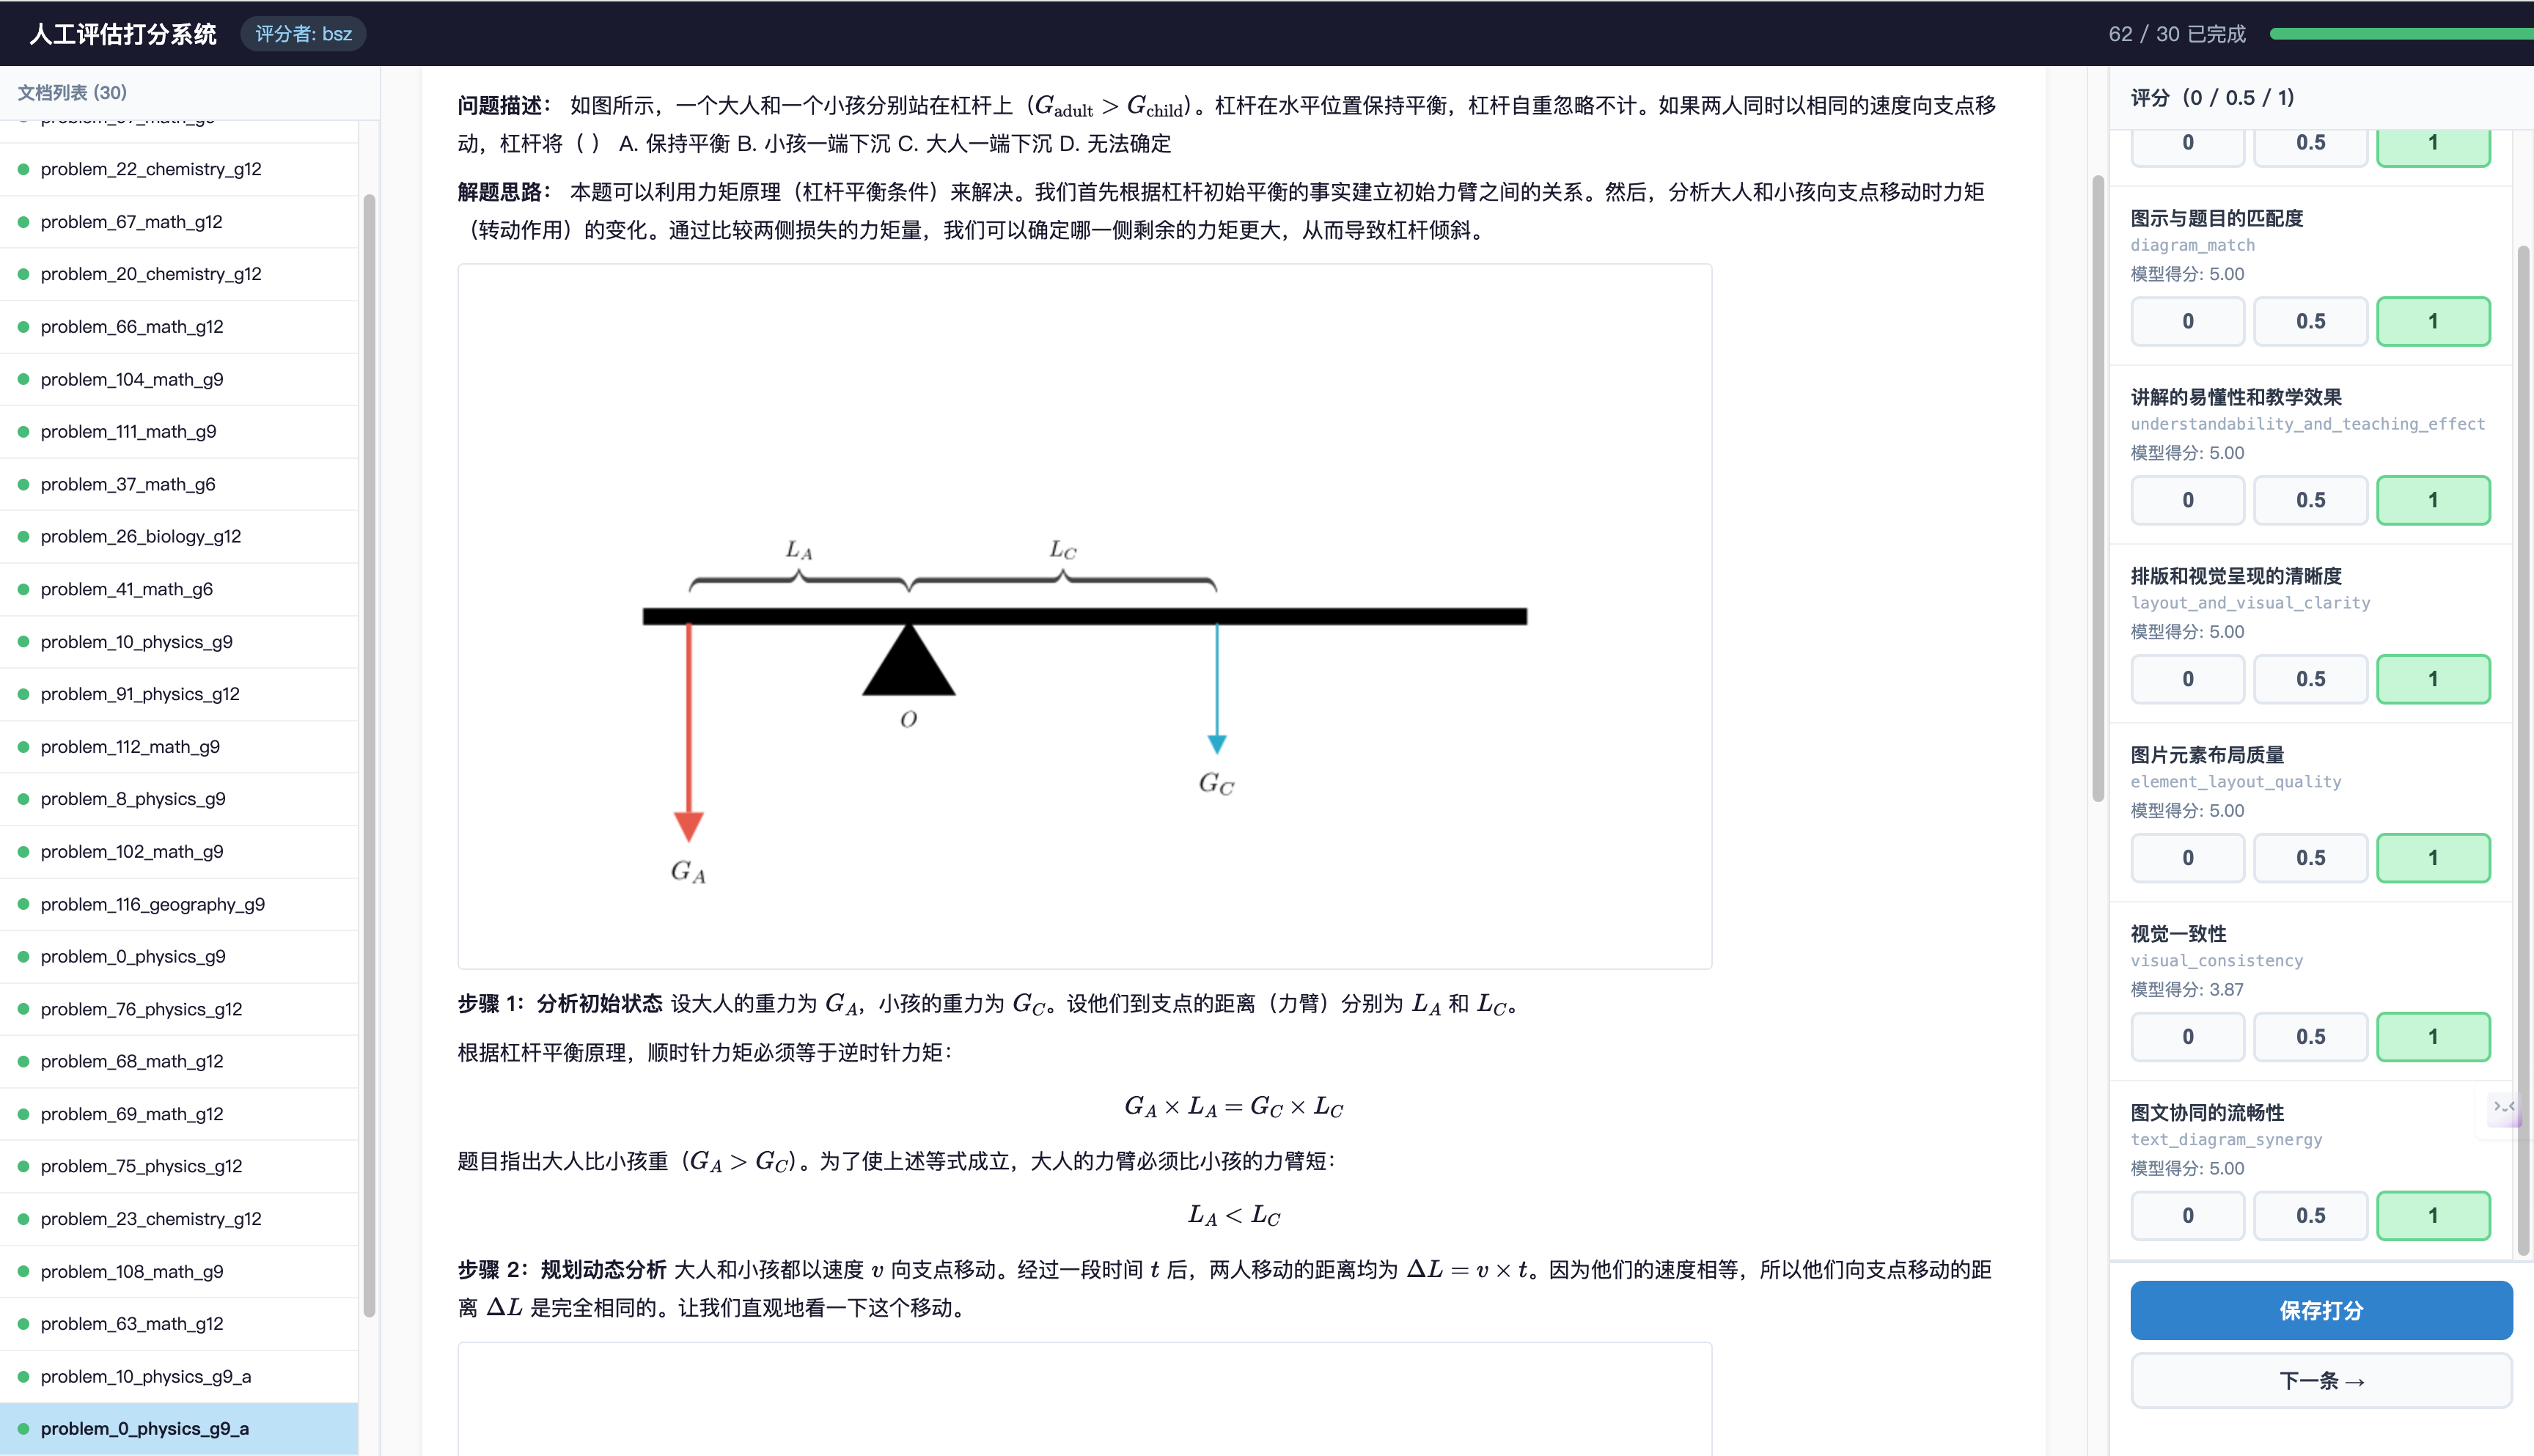
\includegraphics[width=\textwidth]{fig/human_evaluation.png}
  \caption{Screenshot of the human annotation website used for expert evaluation. Raters scored 7 dimensions on a 3-level scale after reviewing the problem, gold solution, and generated explanation with diagrams.}
  \label{fig:annotation}
\end{figure*}
Human evaluation was conducted through a dedicated annotation website. Raters were presented with a K-12 STEM problem, its gold-standard solution, and the generated illustrated explanation (including rendered diagrams). For each explanation, raters scored 7 dimensions (D2--D8) on a coarse 3-level ordinal scale \{0, 0.5, 1\}, where 0 indicates poor quality, 0.5 indicates acceptable quality, and 1 indicates high quality. D1 (Correctness and Completeness) was excluded from human evaluation because solution correctness can be determined objectively by comparing against the gold-standard answer, making subjective human judgment unnecessary and potentially inconsistent. Each page displayed one explanation at a time, with the rubric description and score criteria shown alongside. Raters could zoom into individual diagrams before scoring visual dimensions.

\textbf{Rater Training.} Before formal scoring, all 20 raters underwent a calibration session. For each of the 7 dimensions, we presented two anchor examples---one high-quality explanation demonstrating exemplary visual and textual clarity, and one low-quality explanation exhibiting common failure modes (e.g., overlapping diagram elements, misaligned labels, or pedagogically ineffective step sequencing). Particular emphasis was placed on the aesthetic dimensions (D5 Element Layout Quality and D6 Visual Consistency), as these proved most subjective. Raters discussed borderline cases together to align their interpretation of the 3-level scale.

\textbf{Pilot Scoring.} Following training, raters completed a pilot round on 5 held-out explanations not included in the final evaluation set. Inter-rater agreement was computed via Krippendorff's $\alpha$ after the pilot. Raters whose individual agreement with the group fell below an acceptable threshold were given additional feedback before proceeding. The pilot Krippendorff's $\alpha$ across all dimensions exceeded 0.60, confirming sufficient calibration to proceed with formal scoring.

\textbf{Formal Scoring.} Each of the 30 explanations in the final evaluation set was independently scored by all 20 raters, producing 30 $\times$ 7 $\times$ 20 = 4{,}200 human judgments. Figure~\ref{fig:annotation} shows a screenshot of the annotation interface.



\end{document}
